\documentclass[10pt]{article}
\usepackage{amsmath}
\usepackage{graphicx}
\usepackage{float}
\usepackage{setspace}
\usepackage{booktabs}

\usepackage{hyperref}

\usepackage[a4paper, total={6in,9in}]{geometry}
\linespread{1.5}

% \usepackage{tabularray}
% \usepackage{float}
% \usepackage{graphicx}
% \usepackage{codehigh}
% \usepackage[normalem]{ulem}
% \UseTblrLibrary{booktabs}
% \UseTblrLibrary{siunitx}
% \newcommand{\tinytableTabularrayUnderline}[1]{\underline{#1}}
% \newcommand{\tinytableTabularrayStrikeout}[1]{\sout{#1}}
% \NewTableCommand{\tinytableDefineColor}[3]{\definecolor{#1}{#2}{#3}}


\usepackage[style=apa]{biblatex}
\addbibresource{ref.bib}

\title{Final Project \\ Technology Economics}
\author{Martin Kapl\'{a}nek, Matou\v{s} Fiala, J\'{a}chym L\'{i}va}
\date{June 2026}

\begin{document}

\maketitle

\section{Introduction}

Large cities all over the world suffer from heavy traffic, recently many of them decided to do something about that using different precautions. Urbanists are trying to come up with ideal solution applicable to every city, which is rather complicated task. The measures to keep the traffic bearable are different; somewhere, subsidizing public transport or shared mobility might work, maybe in combination with making these transport means more reliable and preferable over cars. When this is not enough, more restrictive measures must be used. Recently, many cities implemented congestions tolls in the city centres to financially motivate drivers to switch to other transport means while not banning the entry absolutely. This "kinda" tax can be considered as a external mechanism that accounts for the externality of heavy traffic which would be otherwise not financially "visible". 

In the context of the situation described above and given that the case is highly topical around big cities, we aim to focus on one specific outcome of this policy - the intermodal switch, specifically to shared bikes. Leveraging the unique dataset of New York CitiBike provided, we outline a clear research question: After implementation of the congestion toll in New York, did the commuters switch to shared bikes?

Given the nature of the policy and nature of the data, we employ two quasi-experimental research designs: Regression Discontinuity and Difference in Differences. We selected them to match the situation: the toll was implemented strictly on one day and was effective since and the toll area is strictly separated - this allows us to use both the time and spatial boundary in our methodological approach. 

\section{Literature}

This section provides a concise overview of the relevant transport economics literature. First, we outline the theoretical foundation of congestion pricing and its economic rationale, abstracting from multi-modal substitution. Next, we introduce the benchmark framework for multi-modal travel demand, the Four-Step Model. Finally, we review relevant empirical studies examining the causal links between road pricing, fuel costs, and bikesharing demand.

\cite{vickrey1969congestion} established the congestion theory explaining the economic rationale for congestion pricing. The main mechanism is that the congestion toll internalizes the negative externality imposed on others, formalized in the bottleneck model. In this framework, traffic congestion is represented as a queuing process at a capacity-constrained choke point: each additional driver only experiences their own delay, but their entry into the bottleneck pushes back and delays every subsequent driver behind them. The optimal toll occurs where marginal social cost equals marginal private benefit. \cite{vickrey1969congestion} further suggested that the optimal toll should be time-varying, reflecting peak and off-peak rate differentiation as implemented in NYC.
Importantly, the toll is a non-distortive tax. Unlike conventional fiscal taxes that introduce allocative distortions and deadweight loss, the toll corrects an existing distortion by replacing the deadweight loss of queuing time with a price mechanism, eliminating pure delay without reducing bottleneck capacity. Furthermore, unpriced road access leaves scarce bottleneck capacity underpriced, creating an implicit advantage for private car transport over alternative means of transportation and distorting the modal split away from the social optimum.

Compared to single-dimension congestion pricing, the travel demand modeling literature captures individual travel choices within a broader transportation systems analysis framework \parencite{manheim1979fundamentals,mcnally2007four}. The standard and most commonly used approach in this domain is the sequential Four-Step Model (FSM), which resolves travel demand across four successive stages \parencite{mcnally2007four}. First, trip generation determines total travel volume by estimating the trips produced by households and attracted by destinations. Second, trip distribution links these origins and destinations based on spatial distance and travel costs. Third, mode choice models how travelers divide among competing transport alternatives—such as driving, public transit, or cycling—based on relative travel times and prices. Finally, route assignment allocates these modal trips onto the physical network, establishing a traffic equilibrium that accounts for road congestion and network delay. Because trip generation and distribution are typically inelastic in the short run, the introduction of a congestion toll is expected to operate predominantly through mode choice and route assignment, potentially driving modal substitution toward alternatives such as shared bikes.

One of the most relevant empirical studies is \cite{CORNAGO2023102821}. They studied the impact of a mirror-like policy shock—specifically, the sudden removal of a congestion toll rather than its introduction—on bike-sharing demand in Milan. Exploiting this quasi-experimental setting, they estimated that the removal of the toll led to an approximately 5\% reduction in bike-sharing demand. The authors found that this effect operates primarily through the congestion channel, as increased traffic congestion makes roads less safe and pleasant for cycling. Additionally, several studies find that changes in fuel prices impact bike-sharing ridership, suggesting modal substitution between private automobiles and bike-sharing \parencite{He2020A,Berezvai2024Investigating}

\section{Background and Data}

New York's \emph{congestion pricing} was a long-debated policy of instituting a toll on driving into the very centre of the town: Downtown Manhattan. After years of stalling, the toll went into effect on January 5, 2025 costing \$9 in peak and \$2.25 in off-peak times. The priced area consists of all of Manhattan below 60th street (around the start of Central Park). This specific boundary was chosen to cover the Queensboro bridge terminating at 59th street (this suggests that there should be continuity of covariates in proximity of the boundary which bodes better for RDD than e.g. a NTA region-based boundary). Overall, the policy was seen as successful with car traffic decreasing by 11\%, faster cars and bus commutes and a reduction of noise complaints and serious injuries from car crashes \cite{NYT2026}.

One less explored facet of the toll is the effect on shared bikes. In New York, the most popular provider is CitiBike, a subsidiary of Lyft, with millions of rides per month. The provider publishes data about all rides as Open data \cite{CitiBike2026}, including start and stop station id's and coordinates, start and stop times, type (manual or e-bike) and membership status of user. Numbers of rides started and ended between January 2024 and January 2026 was aggregated by station and day, then connected with NTA region and Borough data from New York's geodata using the \emph{nytgeo} package. For each station in Manhattan, its distance from the toll line was computed as the length of the tangent line to a line denoting 60th street ($-73.958664, 40.759062 \to -73.993499, 40.773593$) multiplied by which side of the line the point was on ($>0 = toll$). This was computed using the \emph{spatial} extension of DuckDB. 

\subsection{Difference in Differences}

Before the DiD estimation, it is beneficial to view the raw data and observe possible trends. We do this using two approaches: Figure \ref{fig:trends_raw} presents the raw data fitted using flexible function, Figure \ref{fig:trends_adj} presents seasonally adjusted data. While the former suffers from extreme seasonality, which makes the potential evaluation of parallel trends hard, the latter shows only the variation the data that is left after adjusting for individual stations and both weekly and monthly characteristics (we do this adjustment by first regressing the weekly rides ended on station-month and week fixed effects; second, we obtain the residuals and use them as the adjusted values). 

The raw figure shows no distinction between the group dynamics before and after the effect, we can observe that indeed the stations inside and outside the toll zone are different even before the toll, but we do not see any substantial change after its introduction. The second figure, using the adjusted residuals, shows some trends. First, it suggests that the parallel trend assumption is satisfied, as the fitted lines are nearly parallel. Second, there is a noticeable change in level of the fitted line after the toll introduction - while the treated zone increases at once, the control group does exactly the opposite, suggesting that there was a switch of where rides ended, consistent with intuitive expectations of the effect. 

\begin{figure}
    \centering
    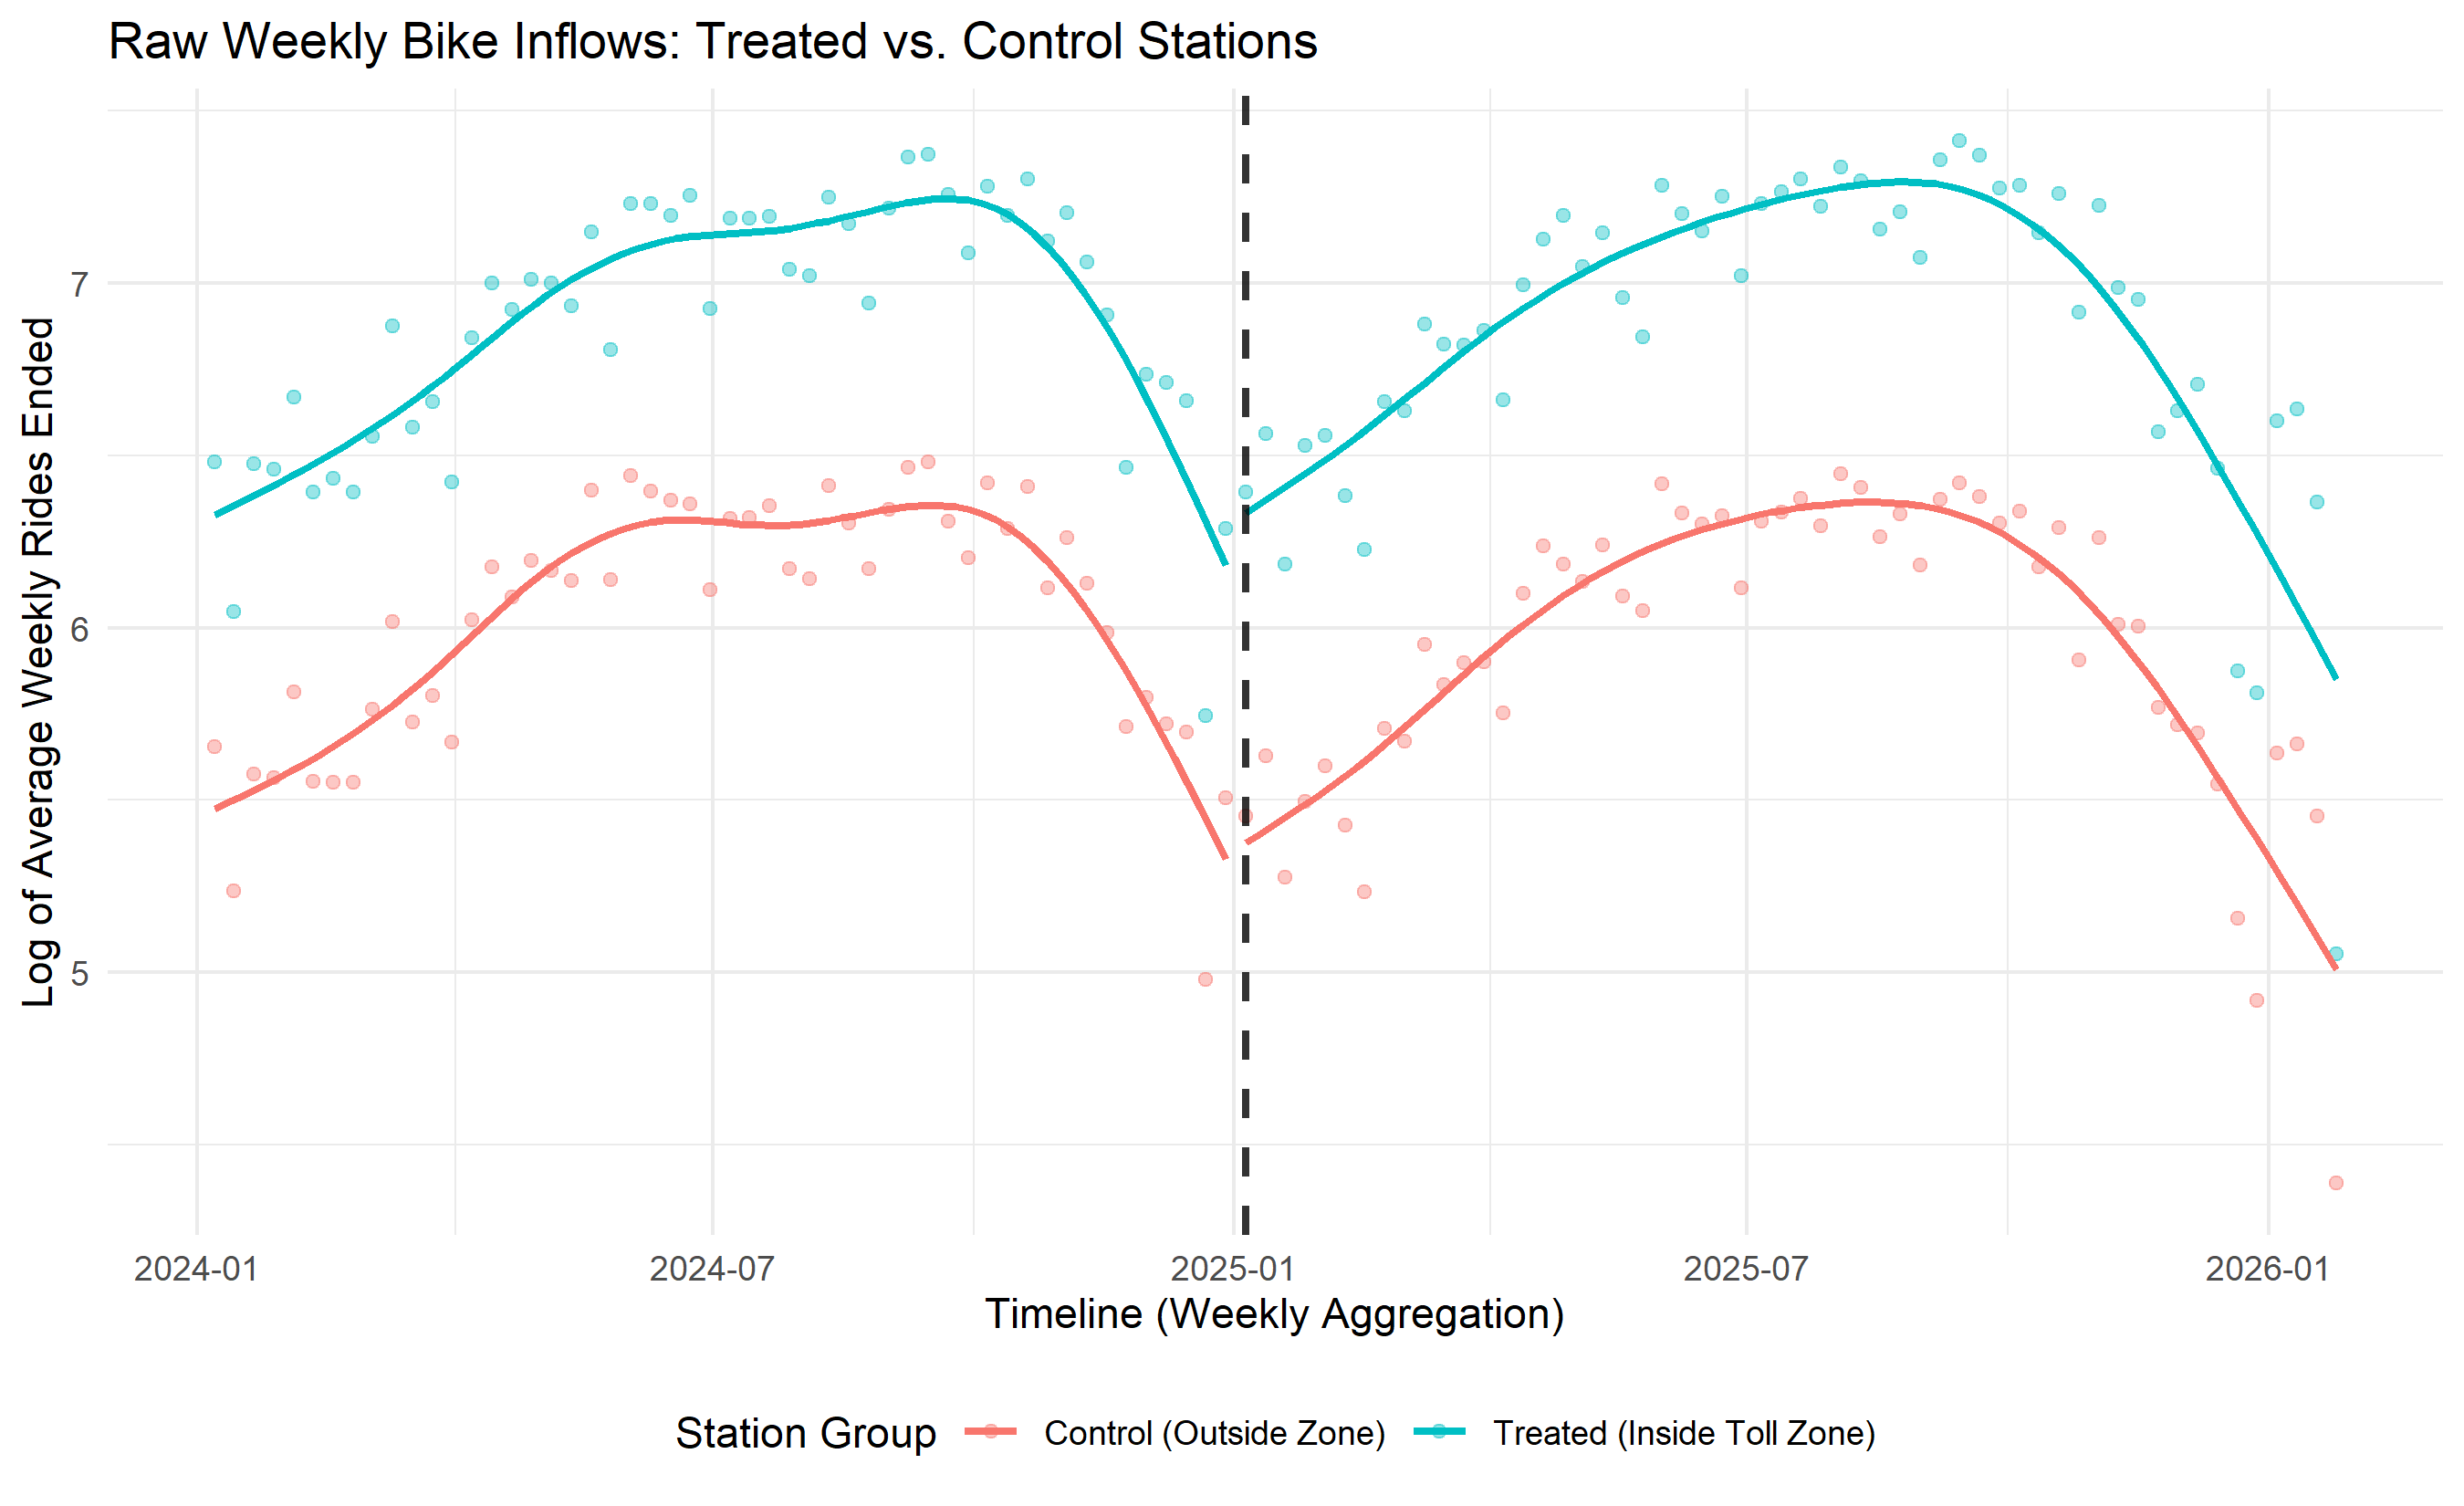
\includegraphics[width=0.9\linewidth]{DiD/outputs/figures/parallel_trends_raw.png}
    \caption{Average log weekly rides ended at treated (inside toll zone) and control (outside zone) stations, January 2024 -- early 2026. GAM smooths are fitted separately for the pre- and post-toll periods (dashed line = January 5, 2025). A strong seasonal pattern dominates both groups; no immediate visual shift is apparent at the toll introduction.}
    \label{fig:trends_raw}
\end{figure}

\begin{figure}
    \centering
    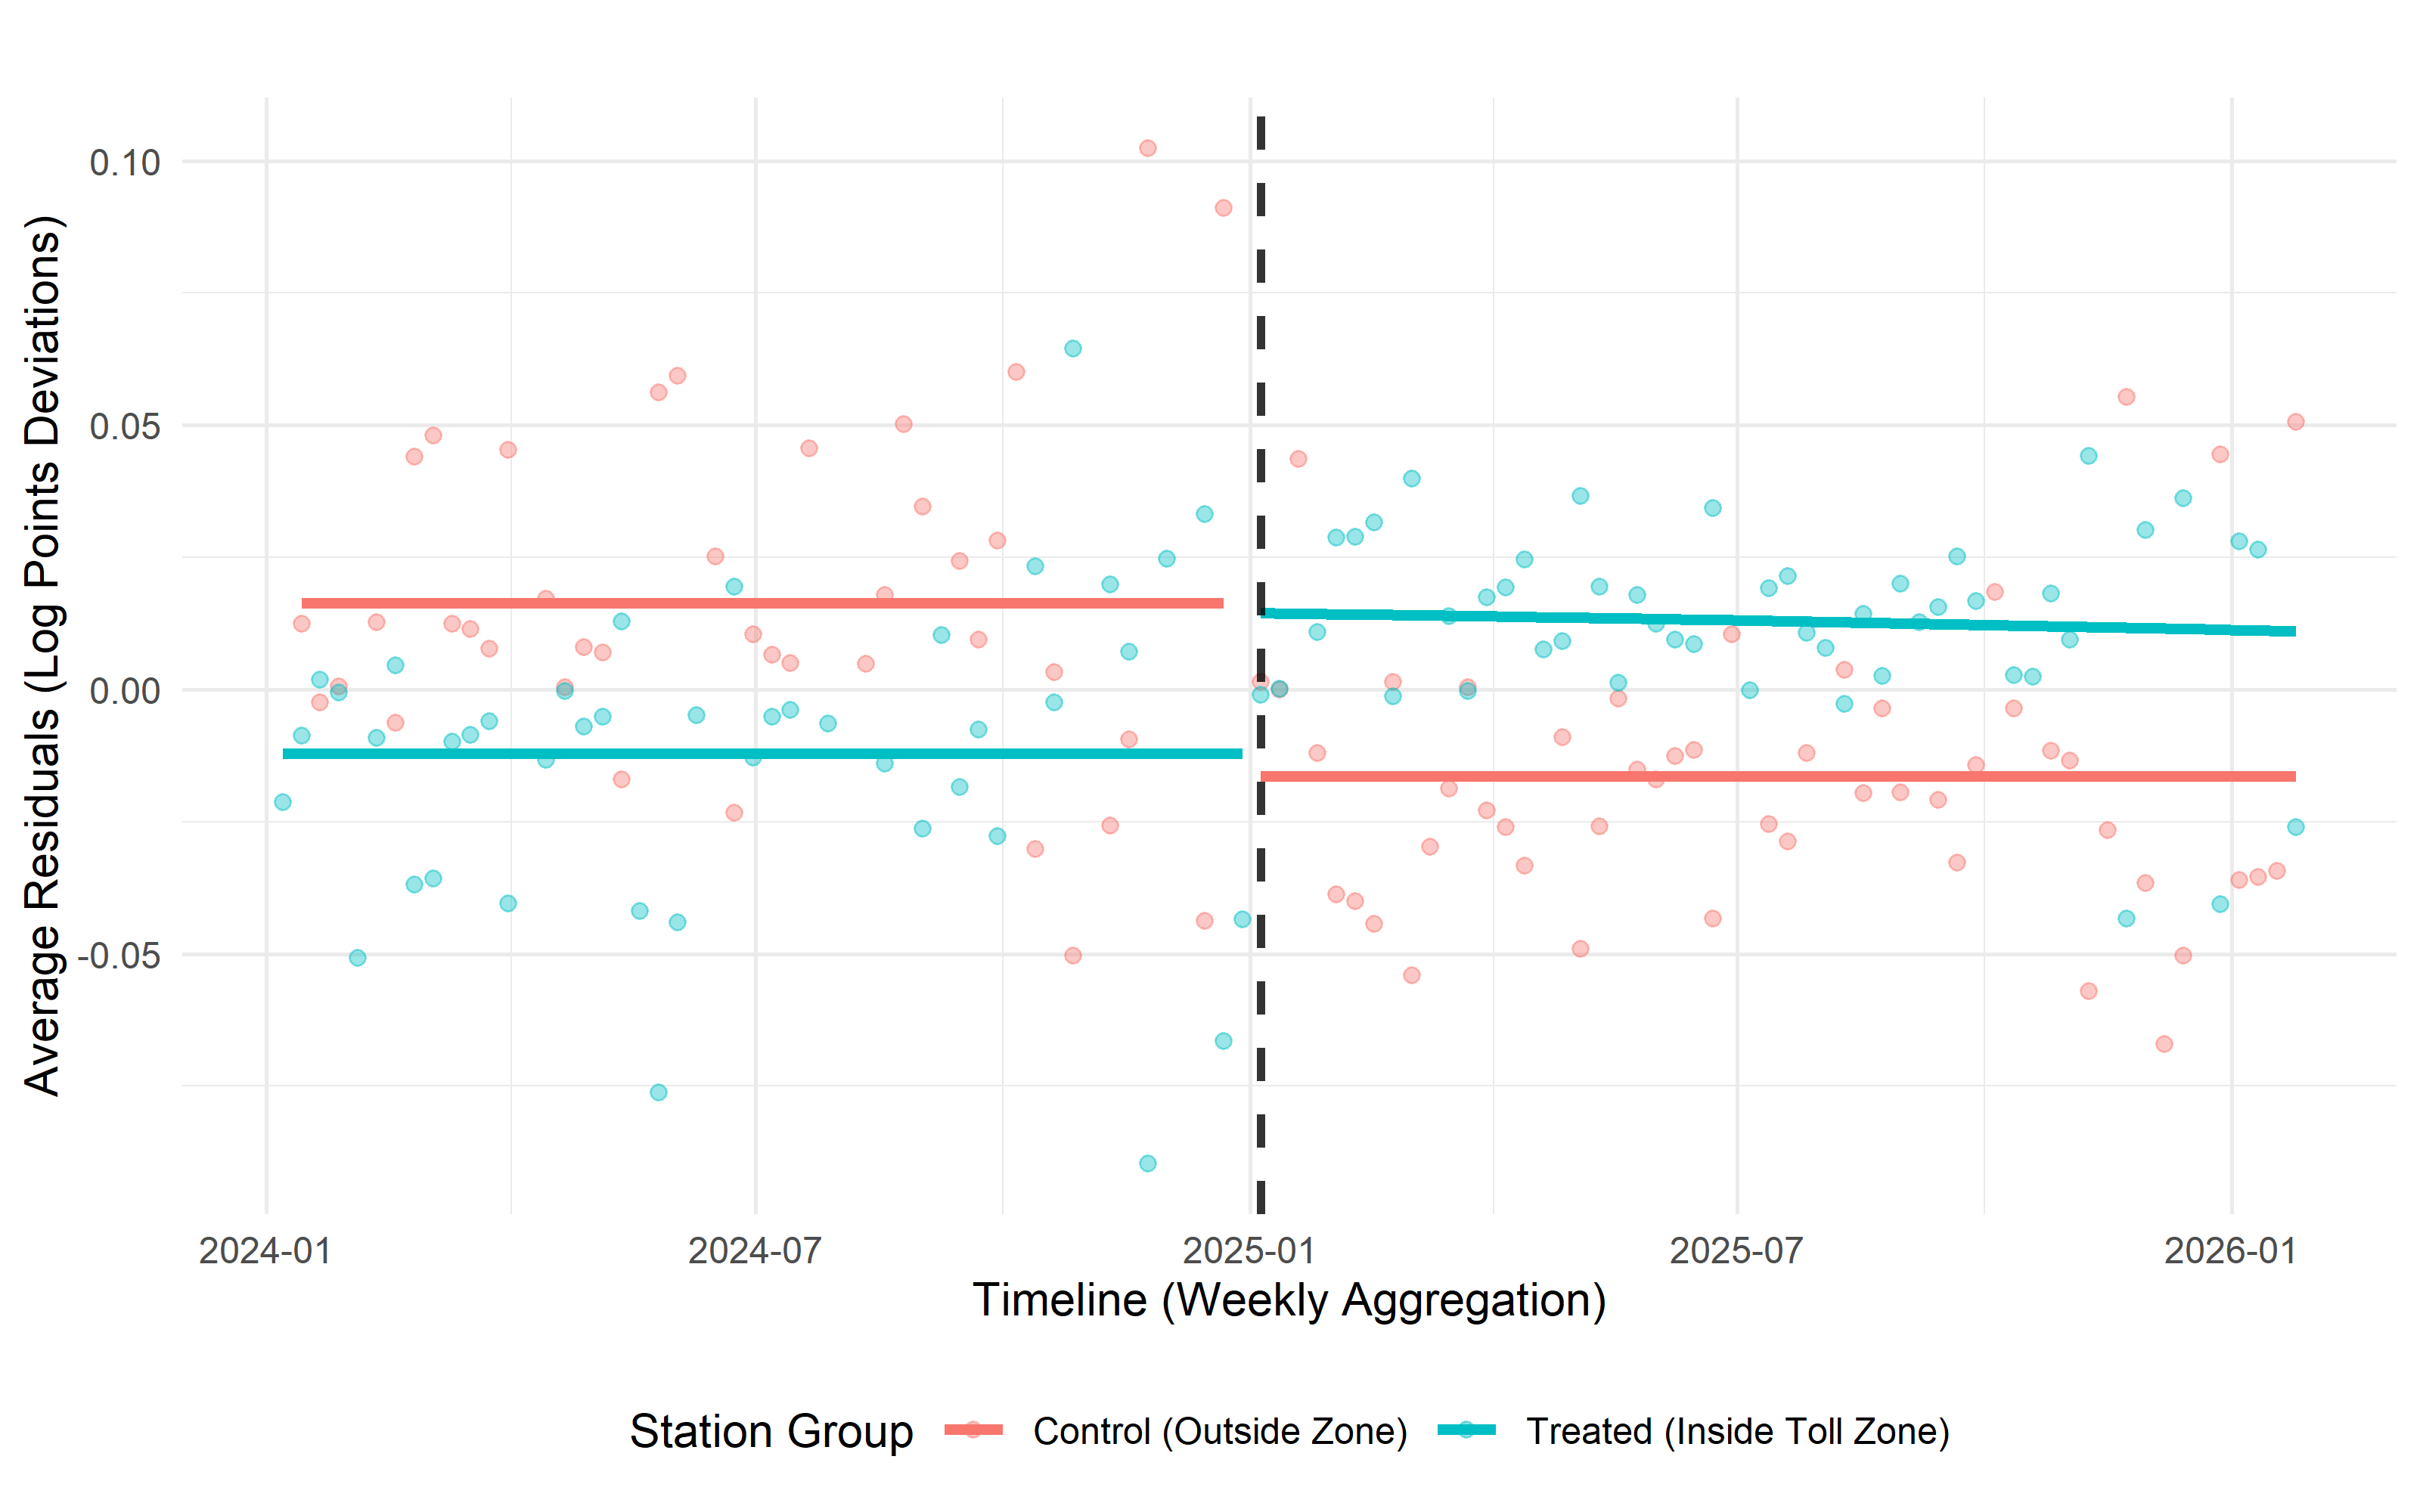
\includegraphics[width=0.9\linewidth]{DiD/outputs/figures/parallel_trends_adjusted.png}
    \caption{Seasonally adjusted parallel trends. Plotted values are residuals from a regression of log weekly rides ended on station$\times$month and week fixed effects. Pre-toll trends are nearly parallel, supporting the parallel trends assumption. A modest upward shift for the treated group is visible immediately after the toll introduction.}
    \label{fig:trends_adj}
\end{figure}

\section{Methodology}

\subsection{Difference in Differences}

We estimate a two-way fixed-effects DiD specification, with the treatment indicator given by the interaction of the toll-zone indicator and a post-toll period indicator (Toll Area $\times$ Post), controlling for station and date (or week, for the weekly aggregation) fixed effects. The outcome variables are rides started (log), rides ended (log), and net inflows (levels), estimated separately at the daily and weekly level as a robustness check across temporal aggregations (Tables \ref{tab:did_static_daily} and \ref{tab:did_static_weekly}). The event studies presented in the Results section are estimated using this same fixed-effect structure.

\subsection{Regression Discontinuity}

The congestion zone boundary is a sharp geographic line that was chosen for reasons unrelated to the continuity assumption of RDD (to include a popular entryway, the Queensboro bridge, into the toll zone). This allows us to isolate the causal effect: a station 100 metres inside and a station 100 metres outside the toll zone should be similar in terms of neighbourhood character, commuting patterns et cetera. The only thing that ought to differ is which side of the line they fall on. If the toll changed behaviour, we should observe a discontinuous jump in outcomes right at the boundary.

The running variable is $X_i$: the signed distance of each station from the toll boundary line. We define the sign so that $X_i > 0$ is inside the toll zone (lower Manhattan and Midtown south of 60th Street) and $X_i < 0$ outside. The cutoff is simply $c = 0$.

To account for any effects of the holiday seasons (i.e. people returning to downtown offices after post-new years holidays regardless of toll), we used a log difference of the station's ridership compared to the same date a year prior:

\begin{equation}
    \Delta Y_i = \log(\text{rides}_{i,\text{Jan 2025}}) - \log(\text{rides}_{i,\text{Jan 2024}})
\end{equation}

\noindent computed over a symmetric $\pm 5$-day window centred on the toll introduction date. Under the assumption that January-to-January changes would have been smooth across the boundary absent the policy, any discontinuity in $\Delta Y_i$ at $c = 0$ can be attributed to the toll.

We estimate the RD effect using local linear regression with a triangular kernel, as implemented in the \texttt{rdrobust} package \cite{Calonico2014}. The bandwidth is chosen by MSE-optimal selection, which balances bias and variance. Inference is based on robust bias-corrected confidence intervals. We separately estimate the discontinuity for rides ended at each station (inflows) and rides started (outflows). The analysis is restricted to Manhattan, since the toll boundary is drawn within that borough and the distance concept loses meaning across the East or Hudson Rivers.

One practical complication deserves mention. Because station locations follow the Manhattan grid, many stations share identical distance values (all stations of 59th street will have an identical euclidian distance from 60th street). \texttt{rdrobust} flags this as mass points in the running variable. We do not expect this to bias the point estimate, but it does inflate uncertainty relative to a completely continuous running variable.

\section{Results}

\subsection{Difference in Differences}

We begin by presenting the event study plots of both rides ended and net rides (Figures \ref{fig:es_monthly_net}, \ref{fig:es_monthly_ended}, \ref{fig:es_weekly_net}, and \ref{fig:es_weekly_ended}). While the net rides show no effect, there is an effect observed for rides ended. But this can be observed on both sides of the figure, suggesting seasonality is playing a role rather than a causal effect of toll introduction.

These visualizations suggest the underlying data might be problematic for DiD estimation, as an effect is detected even before the treatment is applied, this substantially limits the reliability of our results and analysis.

\begin{figure}
    \centering
    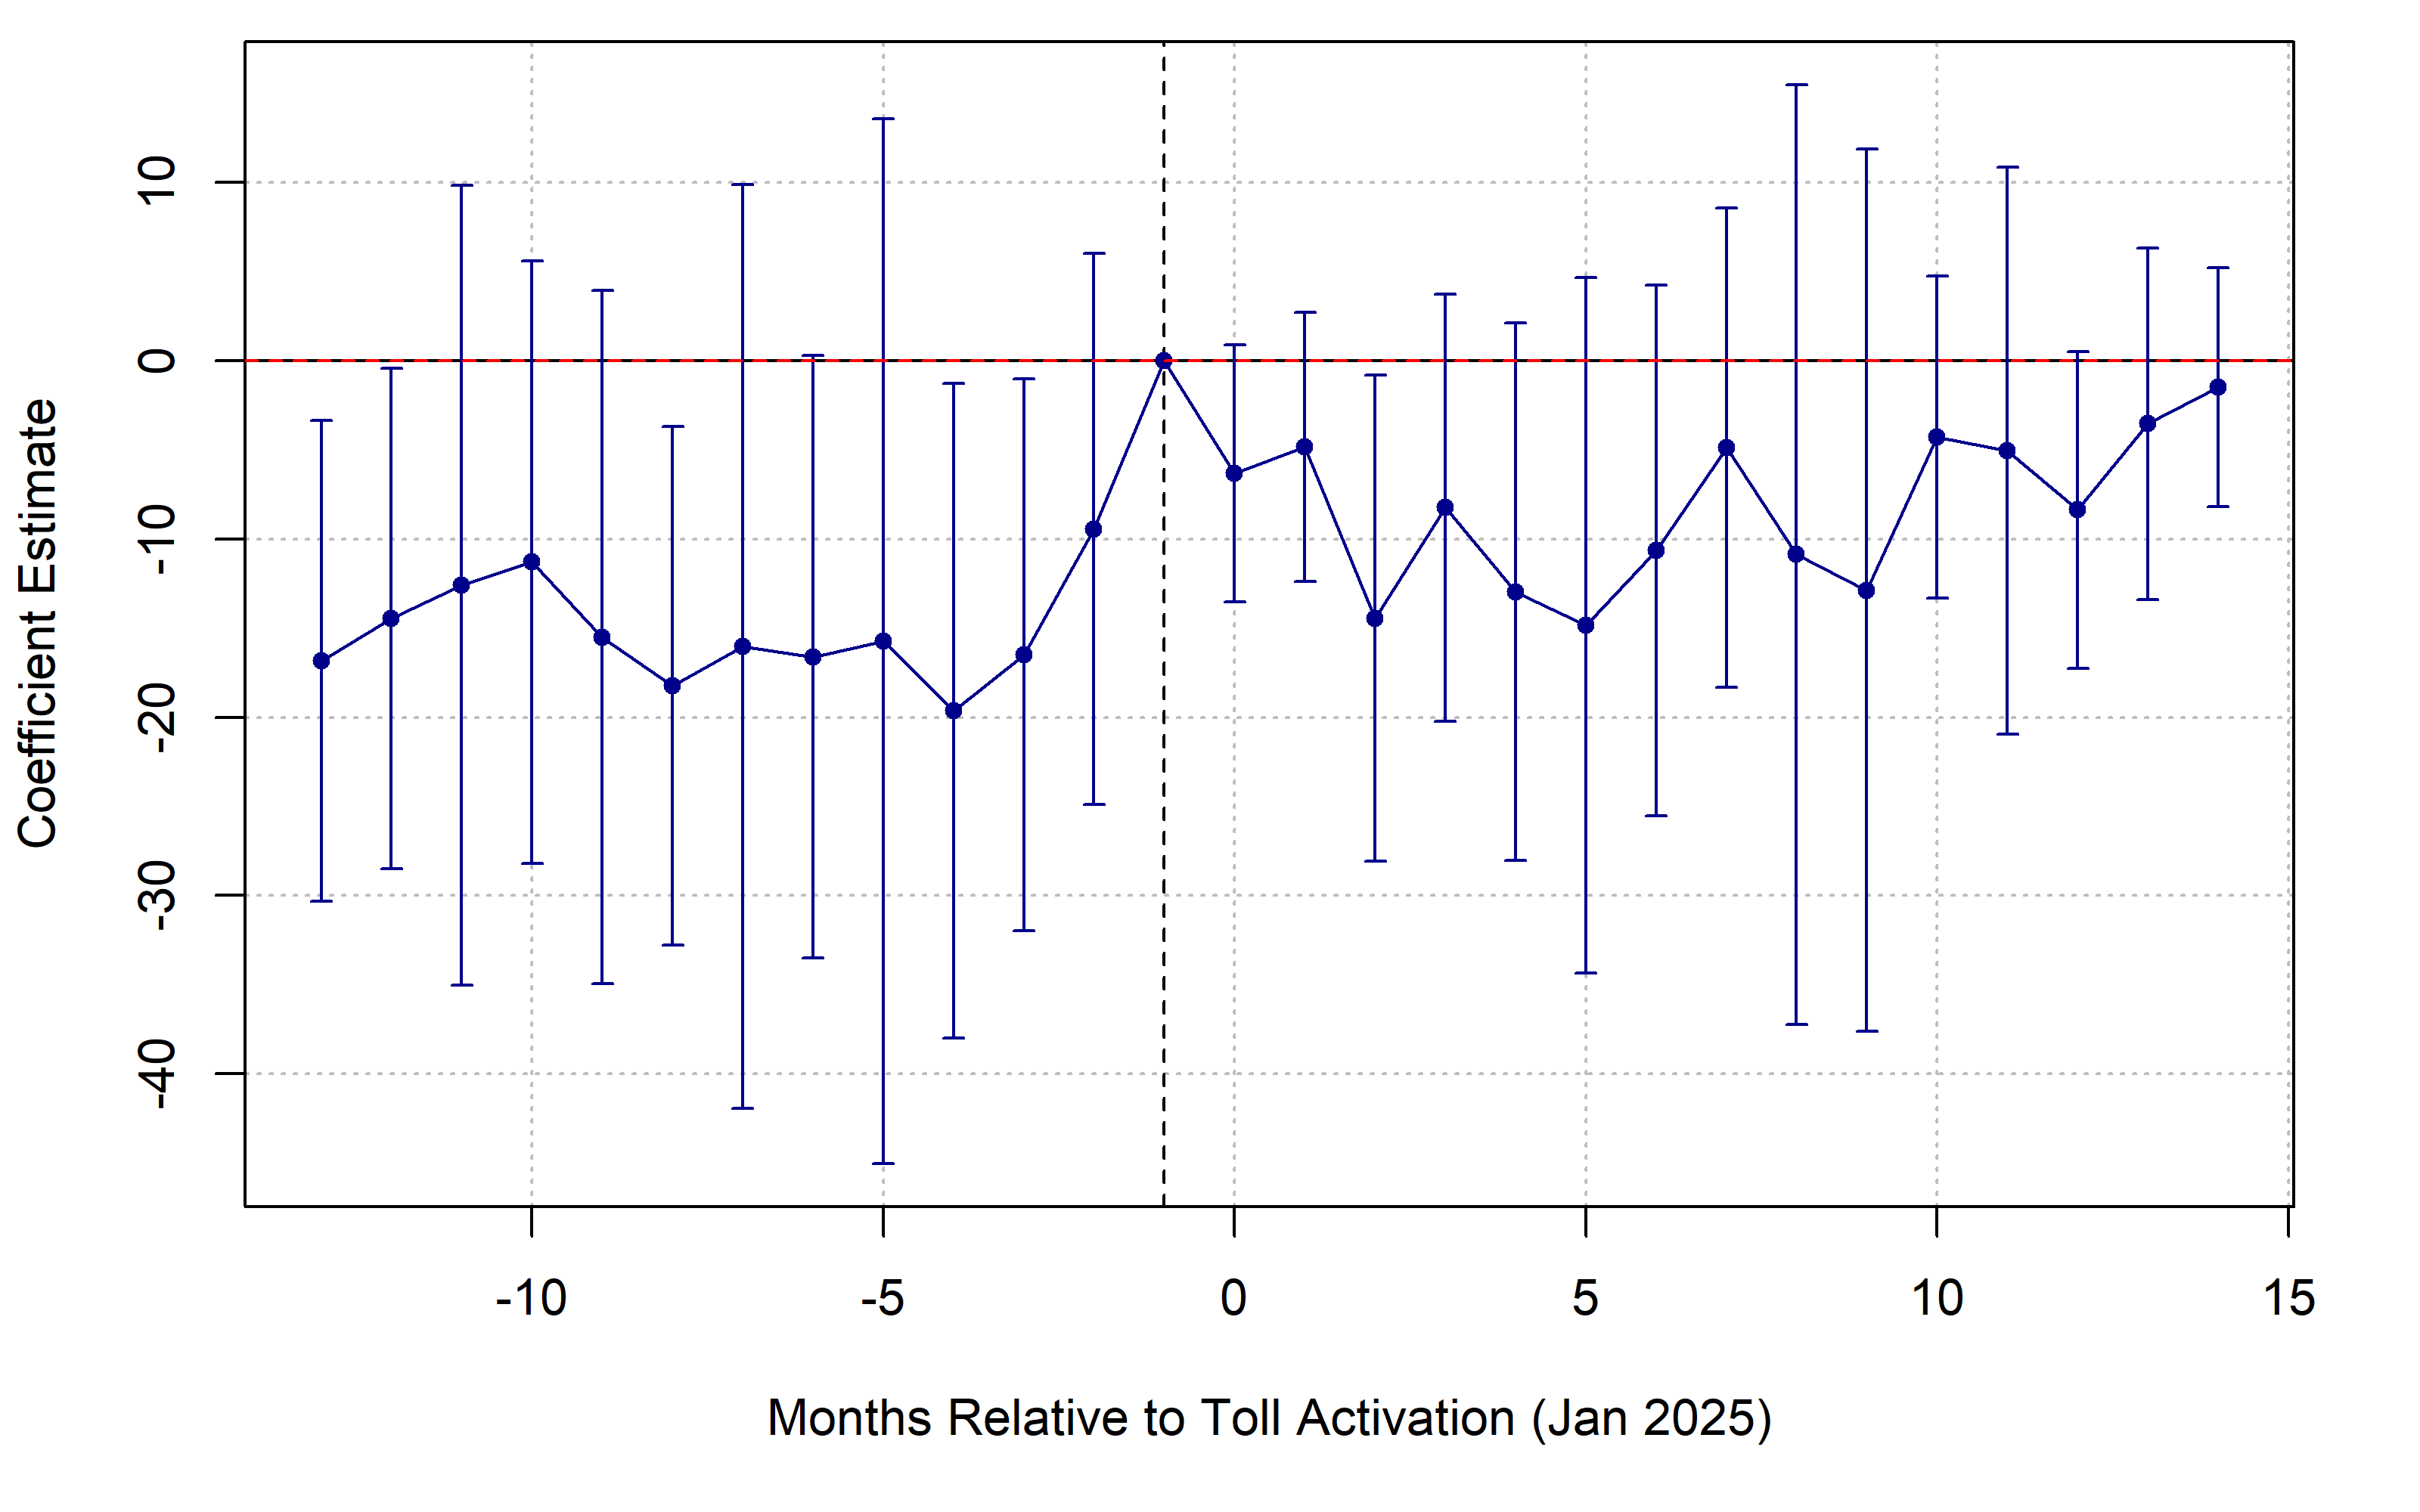
\includegraphics[width=0.9\linewidth]{DiD/outputs/figures/event_study_monthly.png}
    \caption{Event study: net bike inflows (rides ended minus rides started, levels), monthly time units. Coefficients are interactions of the toll-zone indicator with month relative to toll introduction (reference = month $-1$). Estimates are consistently negative both before and after, with wide confidence intervals and no discernible break at month 0.}
    \label{fig:es_monthly_net}
\end{figure}

\begin{figure}
    \centering
    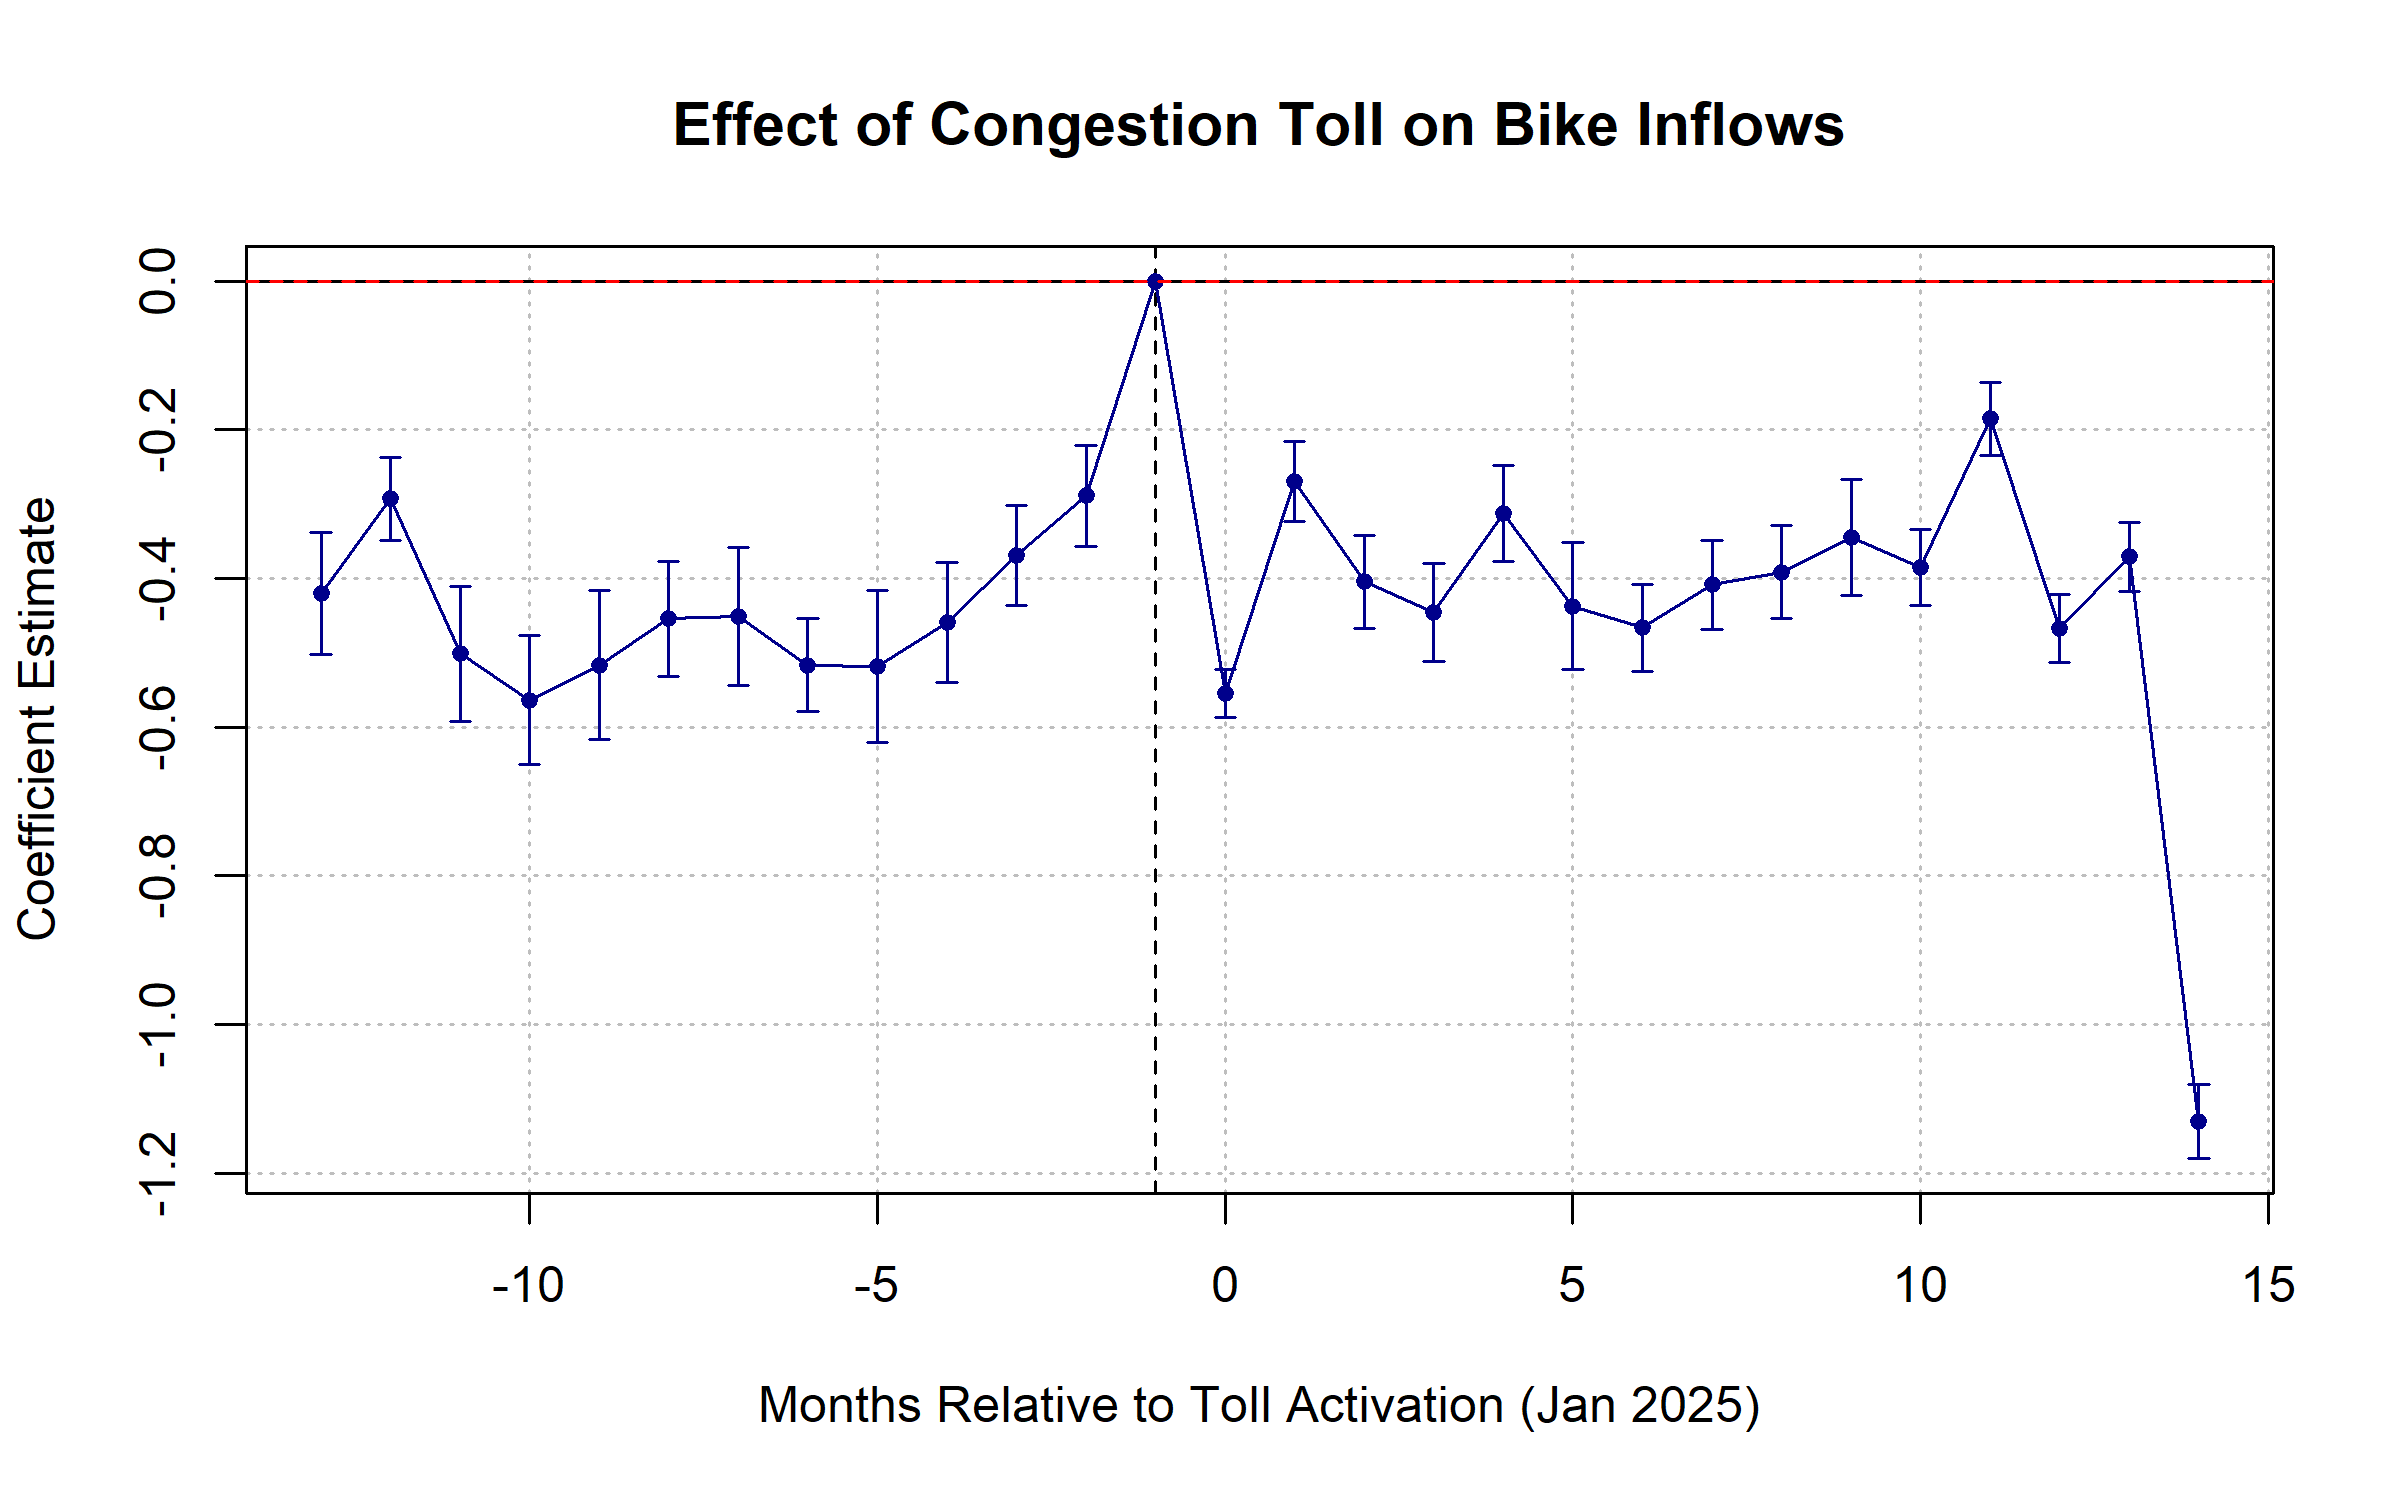
\includegraphics[width=0.9\linewidth]{DiD/outputs/figures/event_study_monthly_ended.png}
    \caption{Event study: log weekly rides ended, monthly time units. Pre-treatment coefficients are systematically negative, suggesting a pre-existing downward trend for treated stations relative to control --- a potential violation of the parallel trends assumption. A small positive spike appears at months 0--1 following the toll introduction.}
    \label{fig:es_monthly_ended}
\end{figure}

\begin{figure}
    \centering
    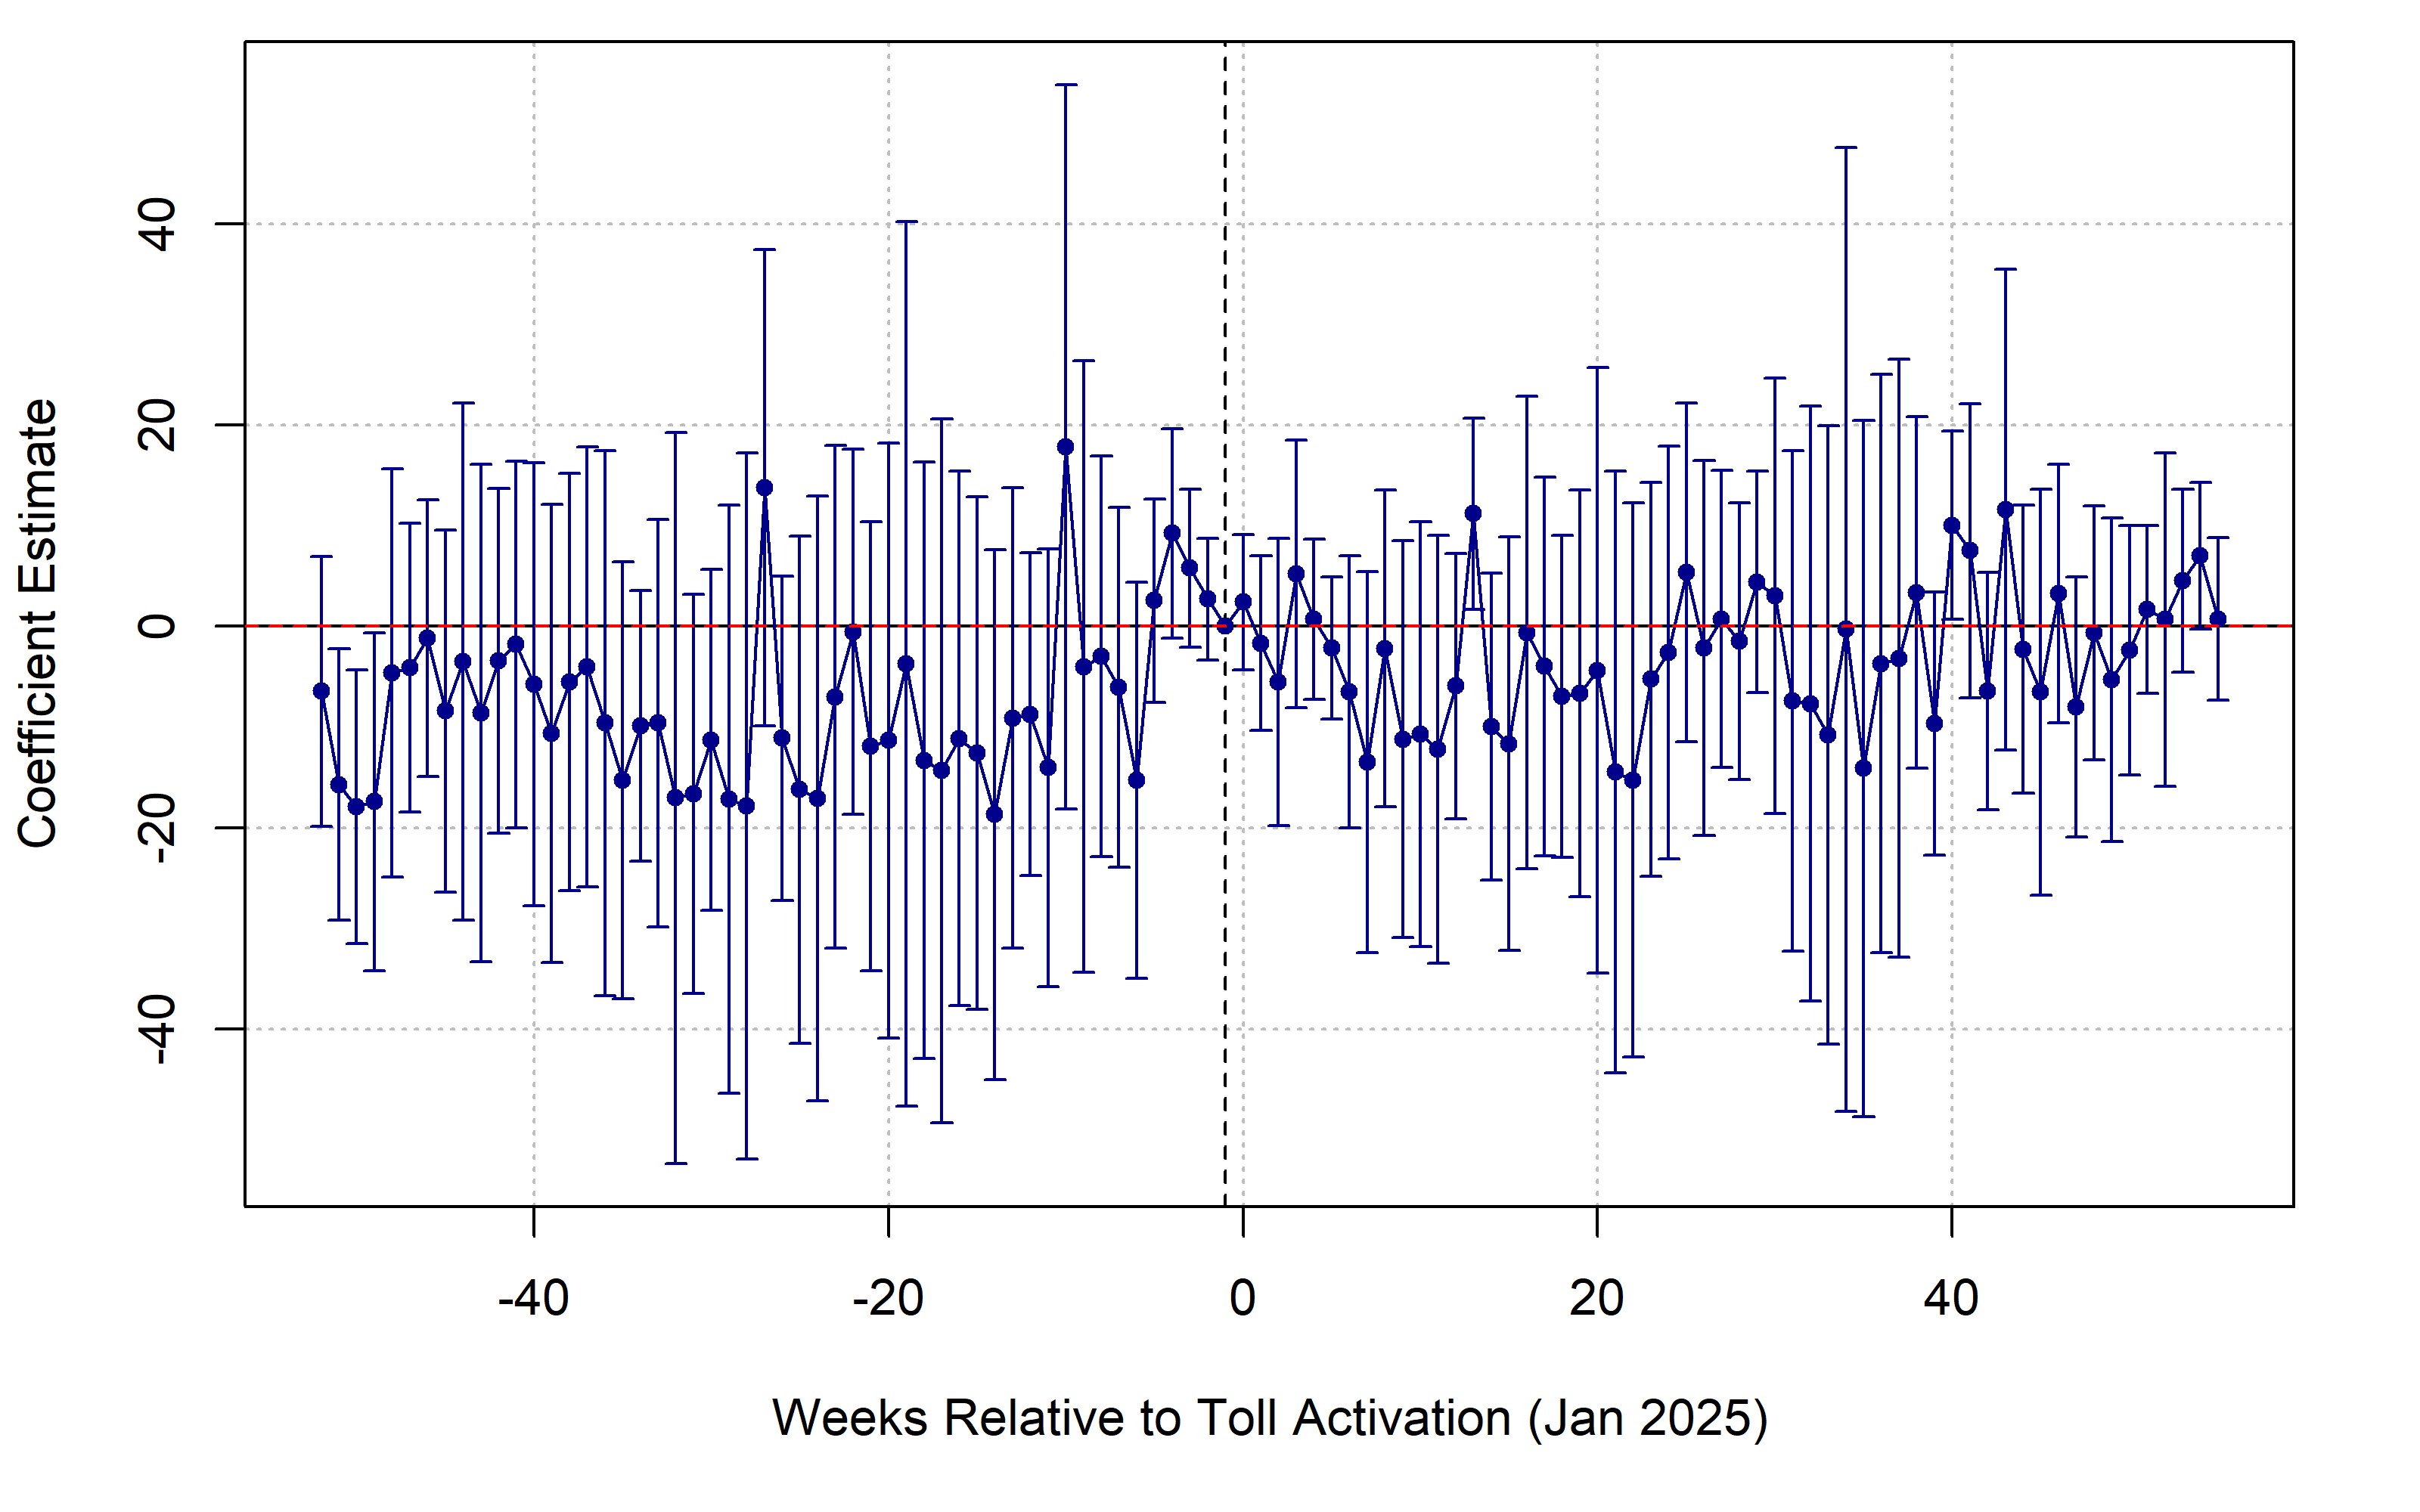
\includegraphics[width=0.9\linewidth]{DiD/outputs/figures/event_study_weekly.png}
    \caption{Event study: net bike inflows (levels), weekly time units. At this resolution the estimates are very noisy; no systematic pre- or post-treatment pattern is discernible.}
    \label{fig:es_weekly_net}
\end{figure}

\begin{figure}
    \centering
    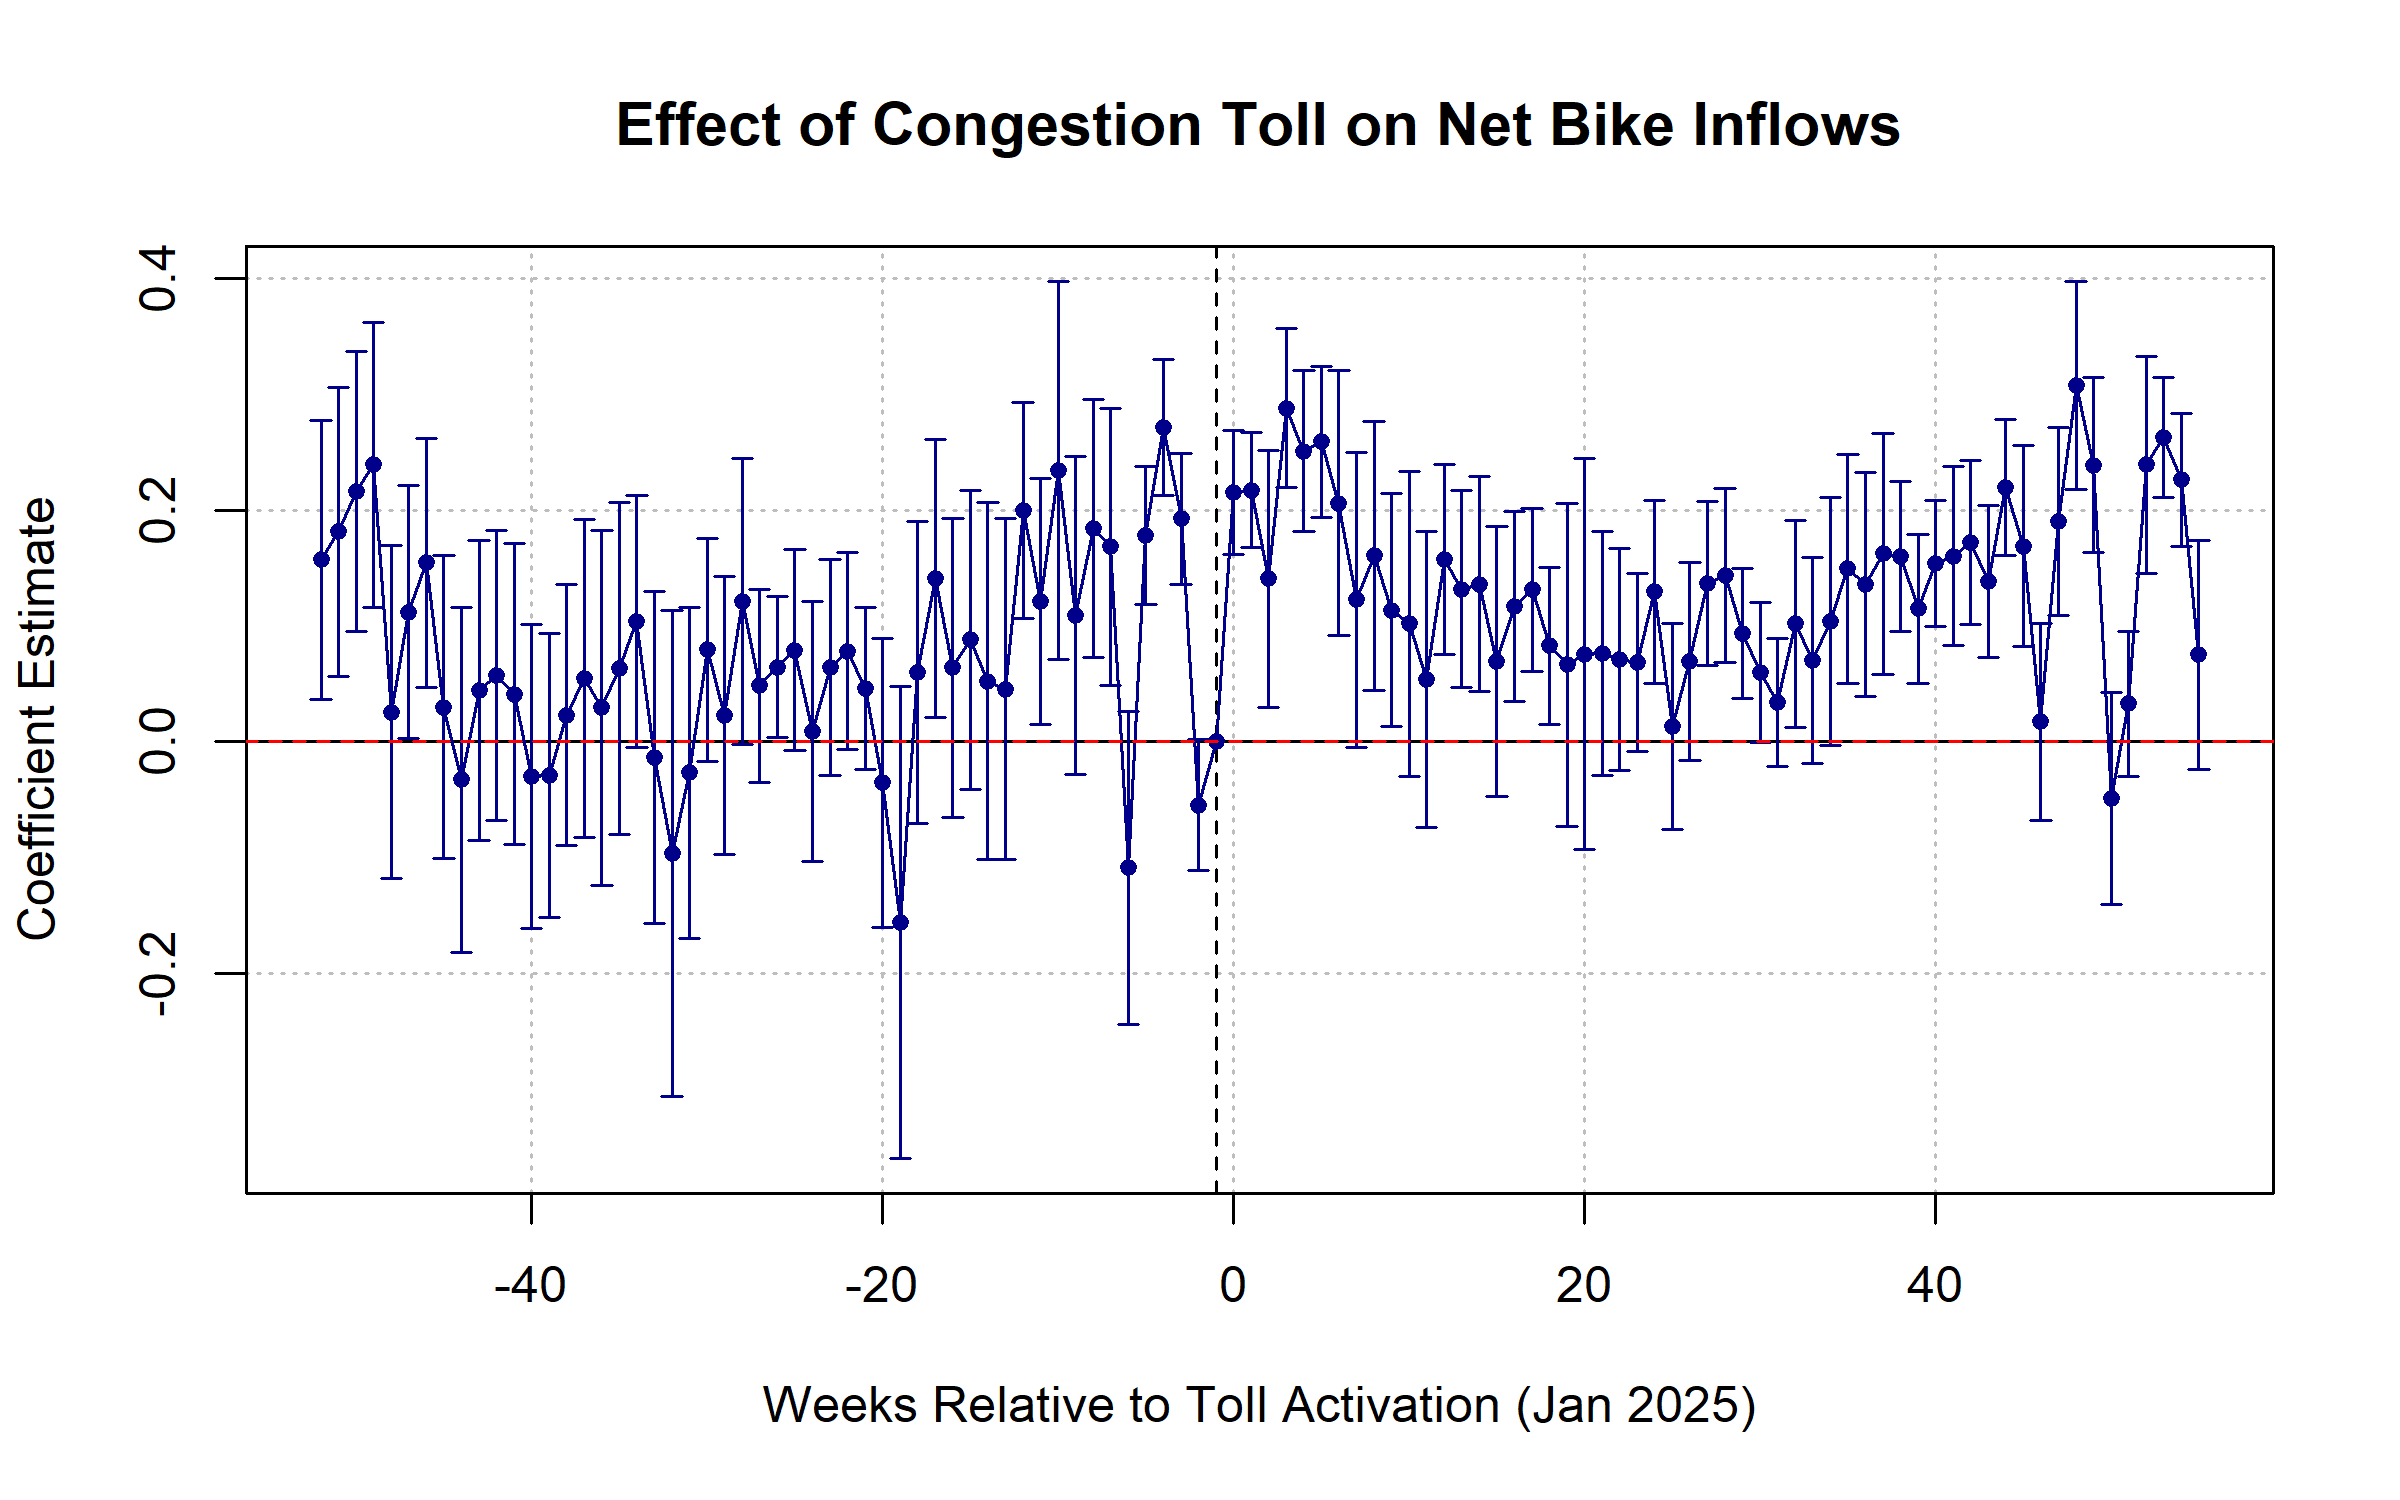
\includegraphics[width=0.9\linewidth]{DiD/outputs/figures/event_study_weekly_ended.png}
    \caption{Event study: log weekly rides ended, weekly time units. Noisy week-by-week estimates; broadly consistent with the monthly picture in Figure~\ref{fig:es_monthly_ended}, with some positive coefficients post-treatment alongside considerable pre-trend variation.}
    \label{fig:es_weekly_ended}
\end{figure}

The results of the preferred models, as shown in Tables \ref{tab:did_static_daily} and \ref{tab:did_static_weekly}, show statistically significant effects for some specifications - namely rides started and ended in logs; for levels, it does not show a significant effect.


\begin{table}[htbp]
   \caption{\label{tab:did_static_daily} Daily Difference-in-Differences Estimates: Congestion Pricing Impact}
   \centering
   \begin{tabular}{lccc}
      \tabularnewline \midrule \midrule
      Dependent Variable:      & Rides Started (Log) & Rides Ended (Log) & Net Inflows (Levels) \\   
      Model:                   & (1)                 & (2)               & (3)\\  
      \midrule
      \emph{Variables}\\
<<<<<<< HEAD
      Toll Area $\times$ Post  & 0.0295              & 0.0495$^{***}$    & 0.4397\\   
                               & (0.0191)            & (0.0154)          & (0.5052)\\   
=======
      Toll Area $\times$ Post  & 0.0588$^{***}$      & 0.0528$^{***}$    & -0.0907\\   
                               & (0.0099)            & (0.0111)          & (0.3500)\\   
>>>>>>> 79c8fe4868f7e652667c510100709347ff9df58c
      \midrule
      \emph{Fixed-effects}\\
      station\_id              & Yes                 & Yes               & Yes\\  
      date                     & Yes                 & Yes               & Yes\\  
      \midrule
      \emph{Fit statistics}\\
<<<<<<< HEAD
      Observations             & 465,276             & 465,276           & 465,276\\  
      R$^2$                    & 0.83102             & 0.81556           & 0.21864\\  
      Adjusted R$^2$           & 0.83050             & 0.81499           & 0.21624\\  
=======
      Observations             & 450,646             & 450,646           & 450,646\\  
      R$^2$                    & 0.82231             & 0.87170           & 0.24011\\  
      Adjusted R$^2$           & 0.82175             & 0.87129           & 0.23770\\  
>>>>>>> 79c8fe4868f7e652667c510100709347ff9df58c
      \midrule \midrule
      \multicolumn{4}{l}{\emph{Clustered (station\_id) standard-errors in parentheses}}\\
      \multicolumn{4}{l}{\emph{Signif. Codes: ***: 0.01, **: 0.05, *: 0.1}}\\
   \end{tabular}
\end{table}



%
\begin{table}[htbp]
   \caption{\label{tab:did_static_daily} Daily Difference-in-Differences Estimates: Congestion Pricing Impact}
   \centering
   \begin{tabular}{lccccc}
      \tabularnewline \midrule \midrule
      Dependent Variable:      & Rides Started (Log) & Rides Ended (Log) & Rides Started (Levels) & Rides Ended (Levels) & Net Inflows (Levels) \\   
      Model:                   & (1)                 & (2)               & (3)                    & (4)                  & (5)\\  
      \midrule
      \emph{Variables}\\
      Toll Area $\times$ Post  & 0.0295              & 0.0495$^{***}$    & 0.4473                 & 0.8869               & 0.4397\\   
                               & (0.0191)            & (0.0154)          & (0.9941)               & (1.047)              & (0.5052)\\   
      \midrule
      \emph{Fixed-effects}\\
      station\_id              & Yes                 & Yes               & Yes                    & Yes                  & Yes\\  
      date                     & Yes                 & Yes               & Yes                    & Yes                  & Yes\\  
      \midrule
      \emph{Fit statistics}\\
      Observations             & 465,276             & 465,276           & 465,276                & 465,276              & 465,276\\  
      R$^2$                    & 0.83102             & 0.81556           & 0.78785                & 0.78918              & 0.21864\\  
      Adjusted R$^2$           & 0.83050             & 0.81499           & 0.78720                & 0.78853              & 0.21624\\  
      \midrule \midrule
      \multicolumn{6}{l}{\emph{Clustered (station\_id) standard-errors in parentheses}}\\
      \multicolumn{6}{l}{\emph{Signif. Codes: ***: 0.01, **: 0.05, *: 0.1}}\\
   \end{tabular}
\end{table}



%
\begin{table}[htbp]
   \caption{\label{tab:did_static_daily} Weekly Difference-in-Differences Estimates: Congestion Pricing Impact}
   \centering
   \begin{tabular}{lccccc}
      \tabularnewline \midrule \midrule
      Dependent Variables:     & log(weekly\_rides\_started)   & log(weekly\_rides\_ended)   & weekly\_rides\_started   & weekly\_rides\_ended   & asinh(weekly\_rides\_net)\\    
      Dependent Variable:      & Rides Started (Log)           & Rides Ended (Log)           & Rides Started (Levels)   & Rides Ended (Levels)   & Net Inflows (Levels) \\   
      Model:                   & (1)                           & (2)                         & (3)                      & (4)                    & (5)\\  
      \midrule
      \emph{Variables}\\
      Toll Area $\times$ Post  & 0.0547$^{***}$                & 0.0562$^{***}$              & 3.665                    & 5.008                  & 0.0036\\   
                               & (0.0091)                      & (0.0098)                    & (7.312)                  & (7.430)                & (0.0891)\\   
      \midrule
      \emph{Fixed-effects}\\
      station\_id              & Yes                           & Yes                         & Yes                      & Yes                    & Yes\\  
      week\_start              & Yes                           & Yes                         & Yes                      & Yes                    & Yes\\  
      \midrule
      \emph{Fit statistics}\\
      Observations             & 56,780                        & 56,780                      & 56,780                   & 56,780                 & 56,780\\  
      R$^2$                    & 0.96125                       & 0.93968                     & 0.88319                  & 0.87032                & 0.21470\\  
      Adjusted R$^2$           & 0.96072                       & 0.93885                     & 0.88159                  & 0.86855                & 0.20396\\  
      -Station Fixed Effects   & Yes                           & Yes                         & Yes                      & Yes                    & Yes\\  
      -Date Fixed Effects      & Yes                           & Yes                         & Yes                      & Yes                    & Yes\\  
      \midrule \midrule
      \multicolumn{6}{l}{\emph{Clustered (station\_id) standard-errors in parentheses}}\\
      \multicolumn{6}{l}{\emph{Signif. Codes: ***: 0.01, **: 0.05, *: 0.1}}\\
   \end{tabular}
\end{table}



\input{DiD/outputs/tables/did_static_weekly}

\subsection{Regression Discontinuity}

Figures \ref{fig:rdd_ended} and \ref{fig:rdd_started} show the RD plots for rides ended and rides started, respectively. Each panel plots binned means of the year-over-year log change against signed distance from the toll boundary, together with local linear fits estimated separately on each side of the cutoff. The dashed vertical line marks the boundary at $X_i = 0$.

\begin{figure}[H]
    \centering
    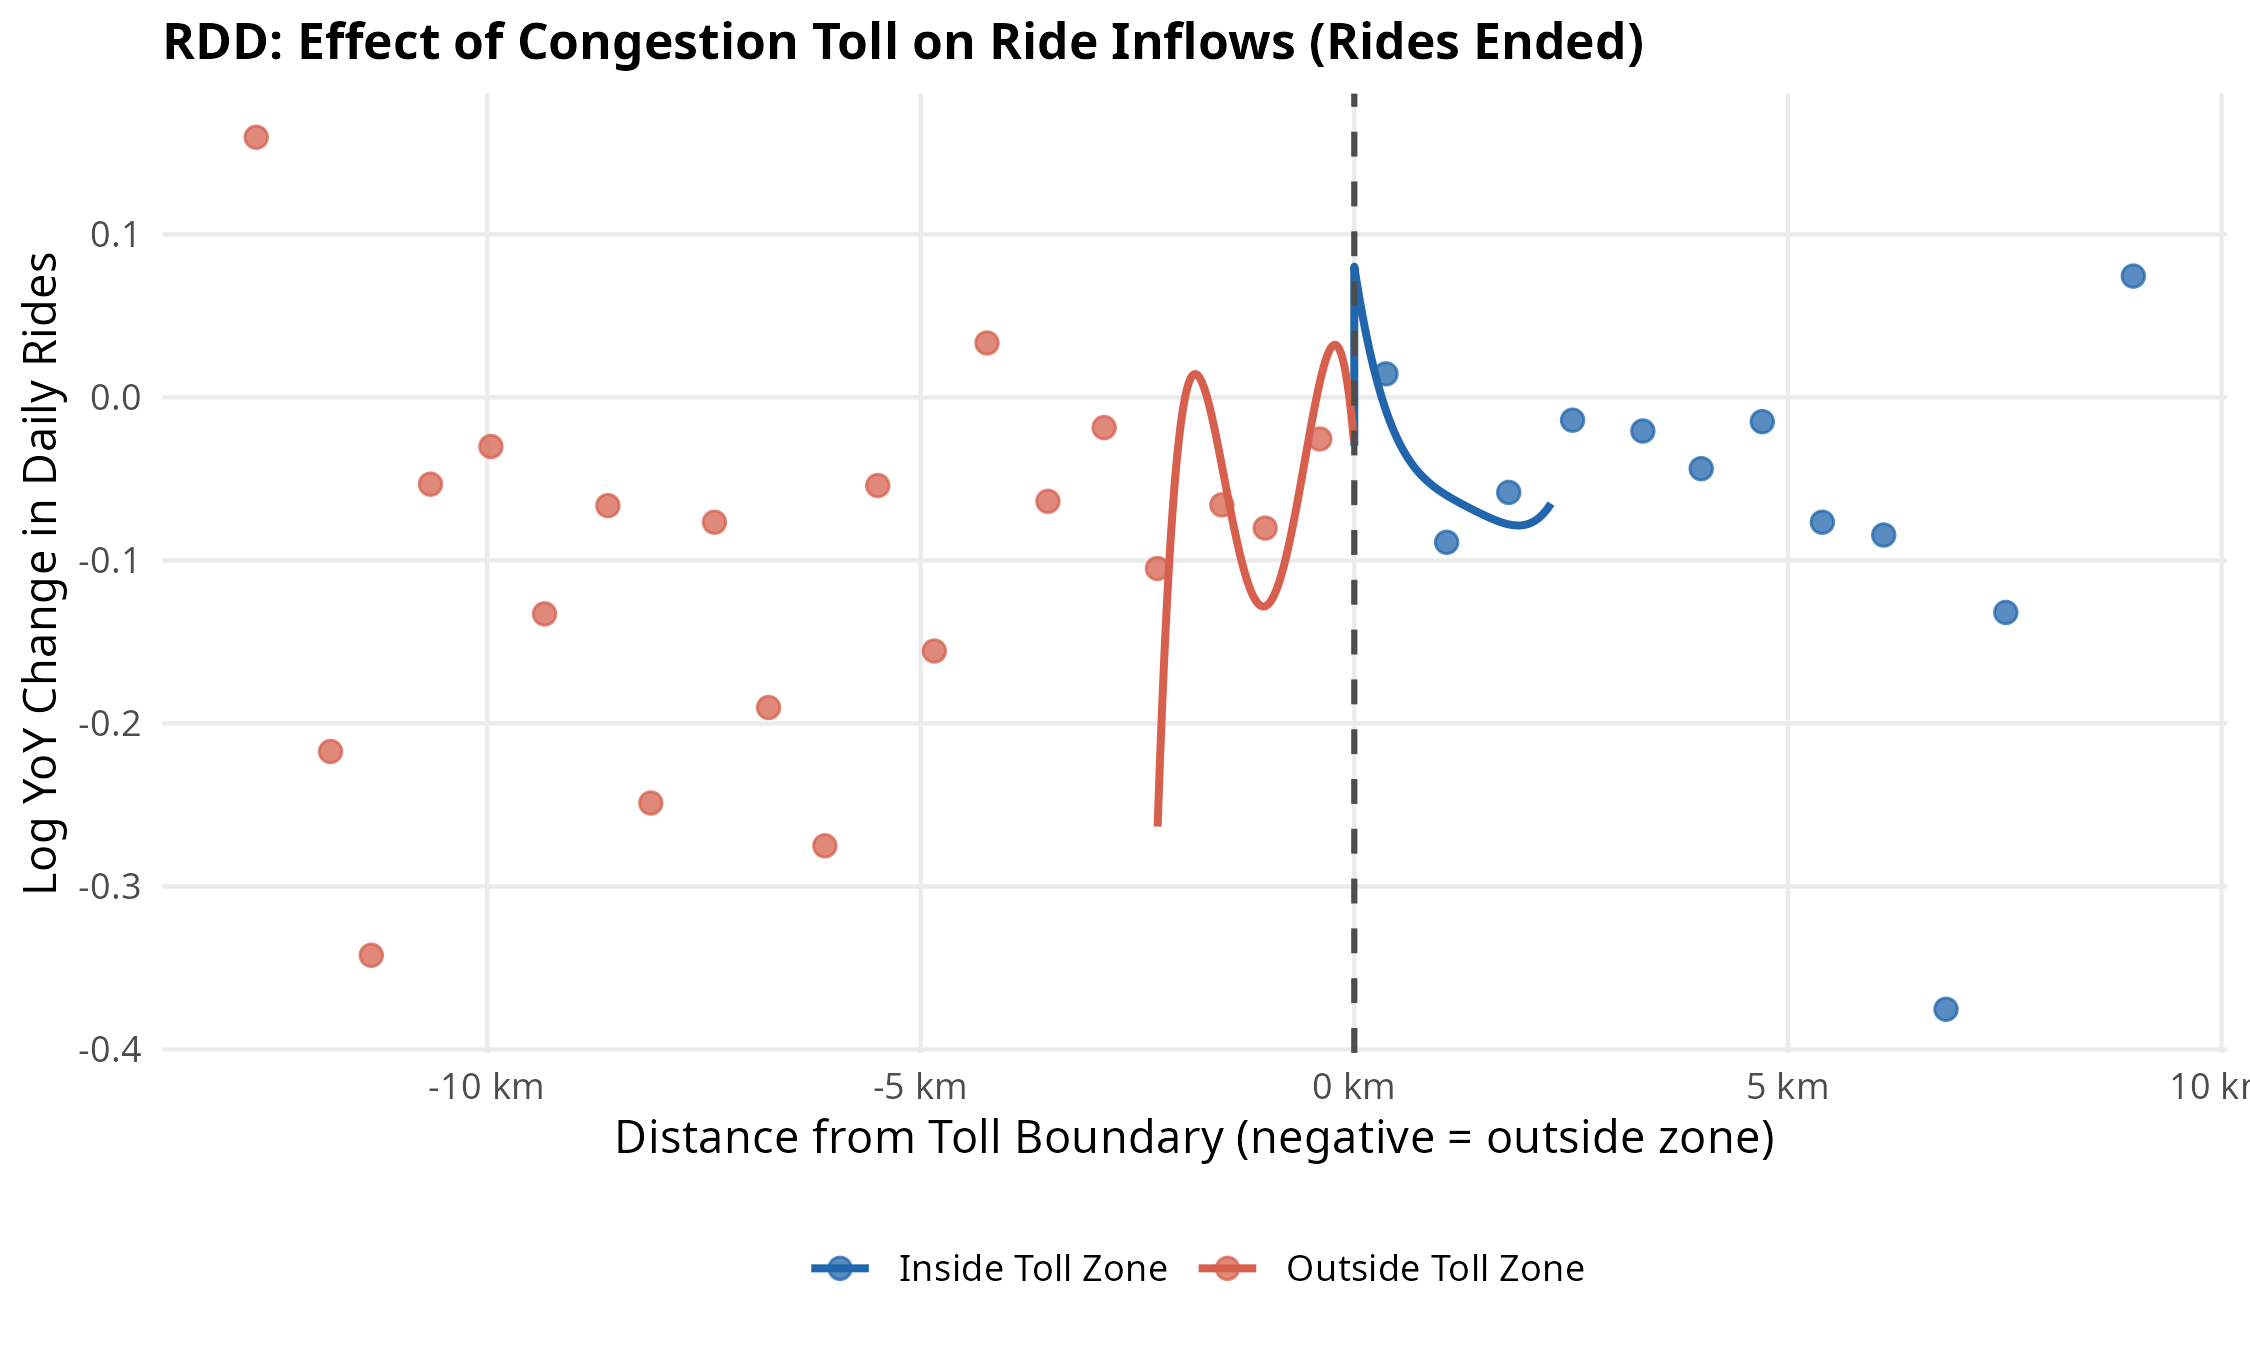
\includegraphics[width=0.9\linewidth]{code/outputs/figures/rdd_rides_ended.png}
    \caption{RD Plot: Log Year-over-Year Change in Rides Ended. Binned means and local linear fits (triangular kernel, MSE-optimal bandwidth) on either side of the toll boundary. Positive signed distance = inside the congestion zone.}
    \label{fig:rdd_ended}
\end{figure}

\begin{figure}[H]
    \centering
    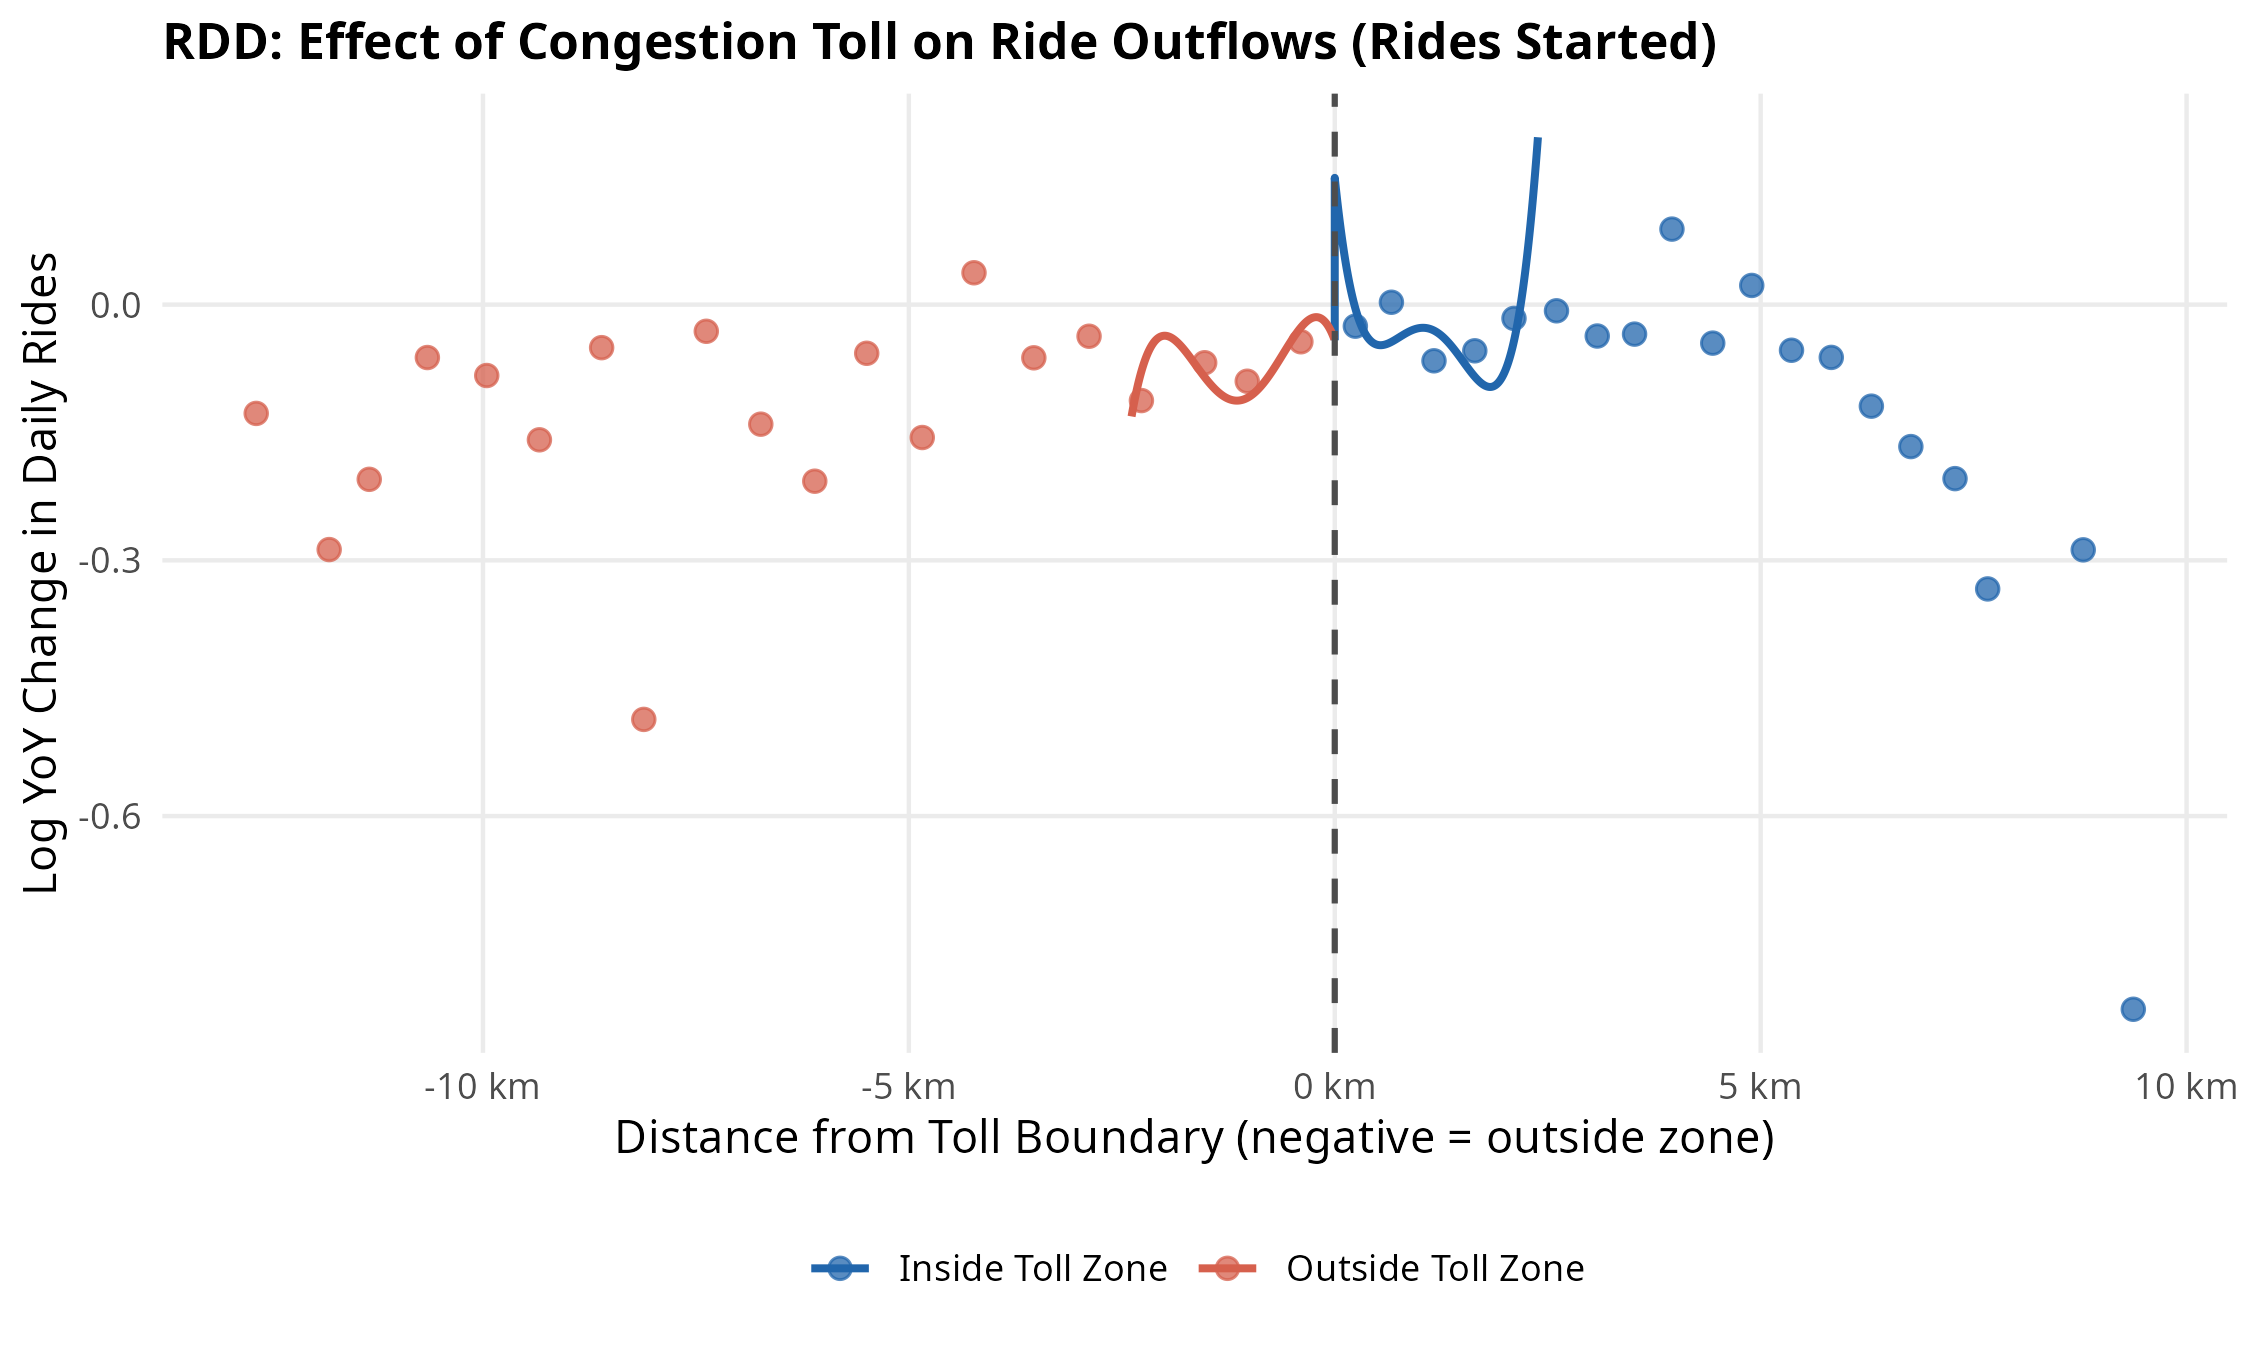
\includegraphics[width=0.9\linewidth]{code/outputs/figures/rdd_rides_started.png}
    \caption{RD Plot: Log Year-over-Year Change in Rides Started. Same specification as Figure \ref{fig:rdd_ended}.}
    \label{fig:rdd_started}
\end{figure}

Neither plot shows a visible jump at the boundary. The fitted lines pass through the cutoff without an obvious discontinuity, and the binned means on either side of zero sit at roughly the same level. This is confirmed by the estimates in Table \ref{tab:rdd_main}. The RD effect for rides ended is 0.023 log points (robust SE = 0.081, $p = 0.760$), and for rides started it is 0.048 log points (robust SE = 0.083, $p = 0.546$). Both confidence intervals are wide and contain zero.


\begin{table}[htbp]
   \caption{\label{tab:rdd_main} Regression Discontinuity Estimates: Congestion Toll Effect}
   \centering
   \begin{tabular}{lcc}
      \tabularnewline \midrule \midrule
                                    & Rides Ended         & Rides Started \\
      Dependent Variable:           & (Log YoY Change)    & (Log YoY Change) \\
      Model:                        & (1)                 & (2)\\
      \midrule
      \emph{Variables}\\
      RD Effect               &  $0.023$           &  $0.048$ \\
                              &  (0.081)             &  (0.083)    \\
      95\% CI               &  $[-0.133,\ 0.183]$  &  $[-0.112,\ 0.212]$ \\
      \midrule
      \emph{Bandwidth \& Sample}\\
      MSE-Optimal Bandwidth (m) &  2268  &  2385 \\
      Effective Observations    &  273  &  285 \\
      \midrule
      \emph{Specification}\\
      Kernel                          & Triangular  & Triangular \\
      Polynomial Order                & 1           & 1 \\
      Inference                       & Robust      & Robust \\
      \midrule \midrule
      \multicolumn{3}{l}{\emph{Robust bias-corrected standard errors in parentheses.}}\\
      \multicolumn{3}{l}{\emph{Signif. Codes: ***: 0.01, **: 0.05, *: 0.1}}\\
   \end{tabular}
\end{table}



The null result contrasts with the DiD, which found a significant positive effect on log rides ended. These designs answer different questions. The DiD uses all treated and control stations and identifies an average effect over time; the RDD is local, recovering the treatment effect only for stations near the boundary. If the toll's impact is concentrated farther inside the zone --- where commuters have no walkable alternative to biking --- stations near the boundary would show little response and the RDD estimate would miss the action entirely.

A further limitation is the presence of mass points in the running variable. Manhattan's grid means that all stations along the same street segment lie at essentially the same perpendicular distance from the toll line, collapsing what should be a continuous running variable into a handful of distinct values. This reduces effective variation and widens standard errors, so the RDD may lack power here rather than identifying a true zero.

\section{Conclusion}

In this project, we analyzed the impact of the implementation of the congestion toll in January 2025 on bike-sharing demand in Manhattan, where the priced zone covers streets up to 60th Street. We used a rich, publicly available dataset from CitiBike, specifically using data from January 2024 to January 2026. We estimated the impact of the congestion toll using two causal inference methods: Difference-in-Differences (DiD) and Regression Discontinuity Design (RDD). In both cases, we used the number of rides (both started and ended) at the station level as the dependent variable. In the regression discontinuity, we used the distance from the boundary of the congestion pricing area as the running variable. We deployed appropriate fixed effects and used various functional forms as robustness checks.

The Difference-in-Differences estimates do not indicate a clear impact, mostly yielding insignificant estimates, although some specifications yield positive estimates for rides ended in logs. However, the event study detects an effect even before the intervention, which substantially limits the reliability of the analysis. The RDD approach did not find a significant causal effect. The RDD approach might be limited by the presence of mass points in the running variable that appear due to the nature of the data, where all points in the same street segment have the same distance from the toll boundary, which can reduce the statistical power of the RDD.

The results suggest that the introduction of tolls is likely not the primary factor that influences bike-sharing demand. To the best of our knowledge, our study is the first to use the RDD approach to estimate the impact of congestion tolls on bike-sharing usage. Due to regional differences, we believe that the external validity of the project is limited. On the other hand, the approach can be used in other cities. Lastly, this project might strongly benefit from an interdisciplinary approach—involving geographic scientists—to improve the methodology as well as the interpretation.

\emph{AI disclosure statement: Agentic and chat tools (Claude; Claude code) were used to consult our methodology, assist with some parts of the code (making plots and tables) and conduct discrete writing tasks (writing out equations in \LaTeX, correcting and editing prose). We take full editorial control and responsibility for the text and the attached code.}

\printbibliography

























\end{document}
